% Generated by Sphinx.
\def\sphinxdocclass{report}
\documentclass[letterpaper,10pt,english]{sphinxmanual}
\usepackage[utf8]{inputenc}
\DeclareUnicodeCharacter{00A0}{\nobreakspace}
\usepackage{cmap}
\usepackage[T1]{fontenc}
\usepackage{babel}
\usepackage{times}
\usepackage[Bjarne]{fncychap}
\usepackage{longtable}
\usepackage{sphinx}
\usepackage{multirow}


\title{RNA-Hi-C-tools Documentation}
\date{June 30, 2014}
\release{0.3.2}
\author{Pengfei Yu}
\newcommand{\sphinxlogo}{}
\renewcommand{\releasename}{Release}
\makeindex

\makeatletter
\def\PYG@reset{\let\PYG@it=\relax \let\PYG@bf=\relax%
    \let\PYG@ul=\relax \let\PYG@tc=\relax%
    \let\PYG@bc=\relax \let\PYG@ff=\relax}
\def\PYG@tok#1{\csname PYG@tok@#1\endcsname}
\def\PYG@toks#1+{\ifx\relax#1\empty\else%
    \PYG@tok{#1}\expandafter\PYG@toks\fi}
\def\PYG@do#1{\PYG@bc{\PYG@tc{\PYG@ul{%
    \PYG@it{\PYG@bf{\PYG@ff{#1}}}}}}}
\def\PYG#1#2{\PYG@reset\PYG@toks#1+\relax+\PYG@do{#2}}

\expandafter\def\csname PYG@tok@gd\endcsname{\def\PYG@tc##1{\textcolor[rgb]{0.63,0.00,0.00}{##1}}}
\expandafter\def\csname PYG@tok@gu\endcsname{\let\PYG@bf=\textbf\def\PYG@tc##1{\textcolor[rgb]{0.50,0.00,0.50}{##1}}}
\expandafter\def\csname PYG@tok@gt\endcsname{\def\PYG@tc##1{\textcolor[rgb]{0.00,0.27,0.87}{##1}}}
\expandafter\def\csname PYG@tok@gs\endcsname{\let\PYG@bf=\textbf}
\expandafter\def\csname PYG@tok@gr\endcsname{\def\PYG@tc##1{\textcolor[rgb]{1.00,0.00,0.00}{##1}}}
\expandafter\def\csname PYG@tok@cm\endcsname{\let\PYG@it=\textit\def\PYG@tc##1{\textcolor[rgb]{0.25,0.50,0.56}{##1}}}
\expandafter\def\csname PYG@tok@vg\endcsname{\def\PYG@tc##1{\textcolor[rgb]{0.73,0.38,0.84}{##1}}}
\expandafter\def\csname PYG@tok@m\endcsname{\def\PYG@tc##1{\textcolor[rgb]{0.13,0.50,0.31}{##1}}}
\expandafter\def\csname PYG@tok@mh\endcsname{\def\PYG@tc##1{\textcolor[rgb]{0.13,0.50,0.31}{##1}}}
\expandafter\def\csname PYG@tok@cs\endcsname{\def\PYG@tc##1{\textcolor[rgb]{0.25,0.50,0.56}{##1}}\def\PYG@bc##1{\setlength{\fboxsep}{0pt}\colorbox[rgb]{1.00,0.94,0.94}{\strut ##1}}}
\expandafter\def\csname PYG@tok@ge\endcsname{\let\PYG@it=\textit}
\expandafter\def\csname PYG@tok@vc\endcsname{\def\PYG@tc##1{\textcolor[rgb]{0.73,0.38,0.84}{##1}}}
\expandafter\def\csname PYG@tok@il\endcsname{\def\PYG@tc##1{\textcolor[rgb]{0.13,0.50,0.31}{##1}}}
\expandafter\def\csname PYG@tok@go\endcsname{\def\PYG@tc##1{\textcolor[rgb]{0.20,0.20,0.20}{##1}}}
\expandafter\def\csname PYG@tok@cp\endcsname{\def\PYG@tc##1{\textcolor[rgb]{0.00,0.44,0.13}{##1}}}
\expandafter\def\csname PYG@tok@gi\endcsname{\def\PYG@tc##1{\textcolor[rgb]{0.00,0.63,0.00}{##1}}}
\expandafter\def\csname PYG@tok@gh\endcsname{\let\PYG@bf=\textbf\def\PYG@tc##1{\textcolor[rgb]{0.00,0.00,0.50}{##1}}}
\expandafter\def\csname PYG@tok@ni\endcsname{\let\PYG@bf=\textbf\def\PYG@tc##1{\textcolor[rgb]{0.84,0.33,0.22}{##1}}}
\expandafter\def\csname PYG@tok@nl\endcsname{\let\PYG@bf=\textbf\def\PYG@tc##1{\textcolor[rgb]{0.00,0.13,0.44}{##1}}}
\expandafter\def\csname PYG@tok@nn\endcsname{\let\PYG@bf=\textbf\def\PYG@tc##1{\textcolor[rgb]{0.05,0.52,0.71}{##1}}}
\expandafter\def\csname PYG@tok@no\endcsname{\def\PYG@tc##1{\textcolor[rgb]{0.38,0.68,0.84}{##1}}}
\expandafter\def\csname PYG@tok@na\endcsname{\def\PYG@tc##1{\textcolor[rgb]{0.25,0.44,0.63}{##1}}}
\expandafter\def\csname PYG@tok@nb\endcsname{\def\PYG@tc##1{\textcolor[rgb]{0.00,0.44,0.13}{##1}}}
\expandafter\def\csname PYG@tok@nc\endcsname{\let\PYG@bf=\textbf\def\PYG@tc##1{\textcolor[rgb]{0.05,0.52,0.71}{##1}}}
\expandafter\def\csname PYG@tok@nd\endcsname{\let\PYG@bf=\textbf\def\PYG@tc##1{\textcolor[rgb]{0.33,0.33,0.33}{##1}}}
\expandafter\def\csname PYG@tok@ne\endcsname{\def\PYG@tc##1{\textcolor[rgb]{0.00,0.44,0.13}{##1}}}
\expandafter\def\csname PYG@tok@nf\endcsname{\def\PYG@tc##1{\textcolor[rgb]{0.02,0.16,0.49}{##1}}}
\expandafter\def\csname PYG@tok@si\endcsname{\let\PYG@it=\textit\def\PYG@tc##1{\textcolor[rgb]{0.44,0.63,0.82}{##1}}}
\expandafter\def\csname PYG@tok@s2\endcsname{\def\PYG@tc##1{\textcolor[rgb]{0.25,0.44,0.63}{##1}}}
\expandafter\def\csname PYG@tok@vi\endcsname{\def\PYG@tc##1{\textcolor[rgb]{0.73,0.38,0.84}{##1}}}
\expandafter\def\csname PYG@tok@nt\endcsname{\let\PYG@bf=\textbf\def\PYG@tc##1{\textcolor[rgb]{0.02,0.16,0.45}{##1}}}
\expandafter\def\csname PYG@tok@nv\endcsname{\def\PYG@tc##1{\textcolor[rgb]{0.73,0.38,0.84}{##1}}}
\expandafter\def\csname PYG@tok@s1\endcsname{\def\PYG@tc##1{\textcolor[rgb]{0.25,0.44,0.63}{##1}}}
\expandafter\def\csname PYG@tok@gp\endcsname{\let\PYG@bf=\textbf\def\PYG@tc##1{\textcolor[rgb]{0.78,0.36,0.04}{##1}}}
\expandafter\def\csname PYG@tok@sh\endcsname{\def\PYG@tc##1{\textcolor[rgb]{0.25,0.44,0.63}{##1}}}
\expandafter\def\csname PYG@tok@ow\endcsname{\let\PYG@bf=\textbf\def\PYG@tc##1{\textcolor[rgb]{0.00,0.44,0.13}{##1}}}
\expandafter\def\csname PYG@tok@sx\endcsname{\def\PYG@tc##1{\textcolor[rgb]{0.78,0.36,0.04}{##1}}}
\expandafter\def\csname PYG@tok@bp\endcsname{\def\PYG@tc##1{\textcolor[rgb]{0.00,0.44,0.13}{##1}}}
\expandafter\def\csname PYG@tok@c1\endcsname{\let\PYG@it=\textit\def\PYG@tc##1{\textcolor[rgb]{0.25,0.50,0.56}{##1}}}
\expandafter\def\csname PYG@tok@kc\endcsname{\let\PYG@bf=\textbf\def\PYG@tc##1{\textcolor[rgb]{0.00,0.44,0.13}{##1}}}
\expandafter\def\csname PYG@tok@c\endcsname{\let\PYG@it=\textit\def\PYG@tc##1{\textcolor[rgb]{0.25,0.50,0.56}{##1}}}
\expandafter\def\csname PYG@tok@mf\endcsname{\def\PYG@tc##1{\textcolor[rgb]{0.13,0.50,0.31}{##1}}}
\expandafter\def\csname PYG@tok@err\endcsname{\def\PYG@bc##1{\setlength{\fboxsep}{0pt}\fcolorbox[rgb]{1.00,0.00,0.00}{1,1,1}{\strut ##1}}}
\expandafter\def\csname PYG@tok@kd\endcsname{\let\PYG@bf=\textbf\def\PYG@tc##1{\textcolor[rgb]{0.00,0.44,0.13}{##1}}}
\expandafter\def\csname PYG@tok@ss\endcsname{\def\PYG@tc##1{\textcolor[rgb]{0.32,0.47,0.09}{##1}}}
\expandafter\def\csname PYG@tok@sr\endcsname{\def\PYG@tc##1{\textcolor[rgb]{0.14,0.33,0.53}{##1}}}
\expandafter\def\csname PYG@tok@mo\endcsname{\def\PYG@tc##1{\textcolor[rgb]{0.13,0.50,0.31}{##1}}}
\expandafter\def\csname PYG@tok@mi\endcsname{\def\PYG@tc##1{\textcolor[rgb]{0.13,0.50,0.31}{##1}}}
\expandafter\def\csname PYG@tok@kn\endcsname{\let\PYG@bf=\textbf\def\PYG@tc##1{\textcolor[rgb]{0.00,0.44,0.13}{##1}}}
\expandafter\def\csname PYG@tok@o\endcsname{\def\PYG@tc##1{\textcolor[rgb]{0.40,0.40,0.40}{##1}}}
\expandafter\def\csname PYG@tok@kr\endcsname{\let\PYG@bf=\textbf\def\PYG@tc##1{\textcolor[rgb]{0.00,0.44,0.13}{##1}}}
\expandafter\def\csname PYG@tok@s\endcsname{\def\PYG@tc##1{\textcolor[rgb]{0.25,0.44,0.63}{##1}}}
\expandafter\def\csname PYG@tok@kp\endcsname{\def\PYG@tc##1{\textcolor[rgb]{0.00,0.44,0.13}{##1}}}
\expandafter\def\csname PYG@tok@w\endcsname{\def\PYG@tc##1{\textcolor[rgb]{0.73,0.73,0.73}{##1}}}
\expandafter\def\csname PYG@tok@kt\endcsname{\def\PYG@tc##1{\textcolor[rgb]{0.56,0.13,0.00}{##1}}}
\expandafter\def\csname PYG@tok@sc\endcsname{\def\PYG@tc##1{\textcolor[rgb]{0.25,0.44,0.63}{##1}}}
\expandafter\def\csname PYG@tok@sb\endcsname{\def\PYG@tc##1{\textcolor[rgb]{0.25,0.44,0.63}{##1}}}
\expandafter\def\csname PYG@tok@k\endcsname{\let\PYG@bf=\textbf\def\PYG@tc##1{\textcolor[rgb]{0.00,0.44,0.13}{##1}}}
\expandafter\def\csname PYG@tok@se\endcsname{\let\PYG@bf=\textbf\def\PYG@tc##1{\textcolor[rgb]{0.25,0.44,0.63}{##1}}}
\expandafter\def\csname PYG@tok@sd\endcsname{\let\PYG@it=\textit\def\PYG@tc##1{\textcolor[rgb]{0.25,0.44,0.63}{##1}}}

\def\PYGZbs{\char`\\}
\def\PYGZus{\char`\_}
\def\PYGZob{\char`\{}
\def\PYGZcb{\char`\}}
\def\PYGZca{\char`\^}
\def\PYGZam{\char`\&}
\def\PYGZlt{\char`\<}
\def\PYGZgt{\char`\>}
\def\PYGZsh{\char`\#}
\def\PYGZpc{\char`\%}
\def\PYGZdl{\char`\$}
\def\PYGZhy{\char`\-}
\def\PYGZsq{\char`\'}
\def\PYGZdq{\char`\"}
\def\PYGZti{\char`\~}
% for compatibility with earlier versions
\def\PYGZat{@}
\def\PYGZlb{[}
\def\PYGZrb{]}
\makeatother

\begin{document}

\maketitle
\tableofcontents
\phantomsection\label{index::doc}


\textbf{Contents:}


\chapter{RNA-Hi-C-tools 0.3 documentation}
\label{RNA-Hi-C-tools:welcome-to-rna-hi-c-tools-s-documentation}\label{RNA-Hi-C-tools::doc}\label{RNA-Hi-C-tools:rna-hi-c-tools-version-documentation}

\section{Overview}
\label{RNA-Hi-C-tools:overview}
\textbf{RNA-Hi-C-tools} is a set of bioinformatic tools for analysis of a novel DNA sequencing based technology to detect RNA-RNA interactome and RNA-chromatin interactome (RNA-chromatin interactome is coming soon).

RNA-HiC-tools automated all the analysis steps, including removing PCR duplicates, splitting multiplexed samples, identifying the linker sequence, splitting junction reads, calling interacting RNAs, statistical assessments, categorizing RNA interaction types, calling interacting sites, and RNA structure analysis, as well as visualization tools for the RNA interactome ({\hyperref[Visualization:visualizationglobal]{\emph{Visualization of global interactome}}}) and the proximal sites within an RNA ({\hyperref[Visualization:visualizationheatmap]{\emph{Heatmap for Intra-RNA interactions}}}).

{\hfill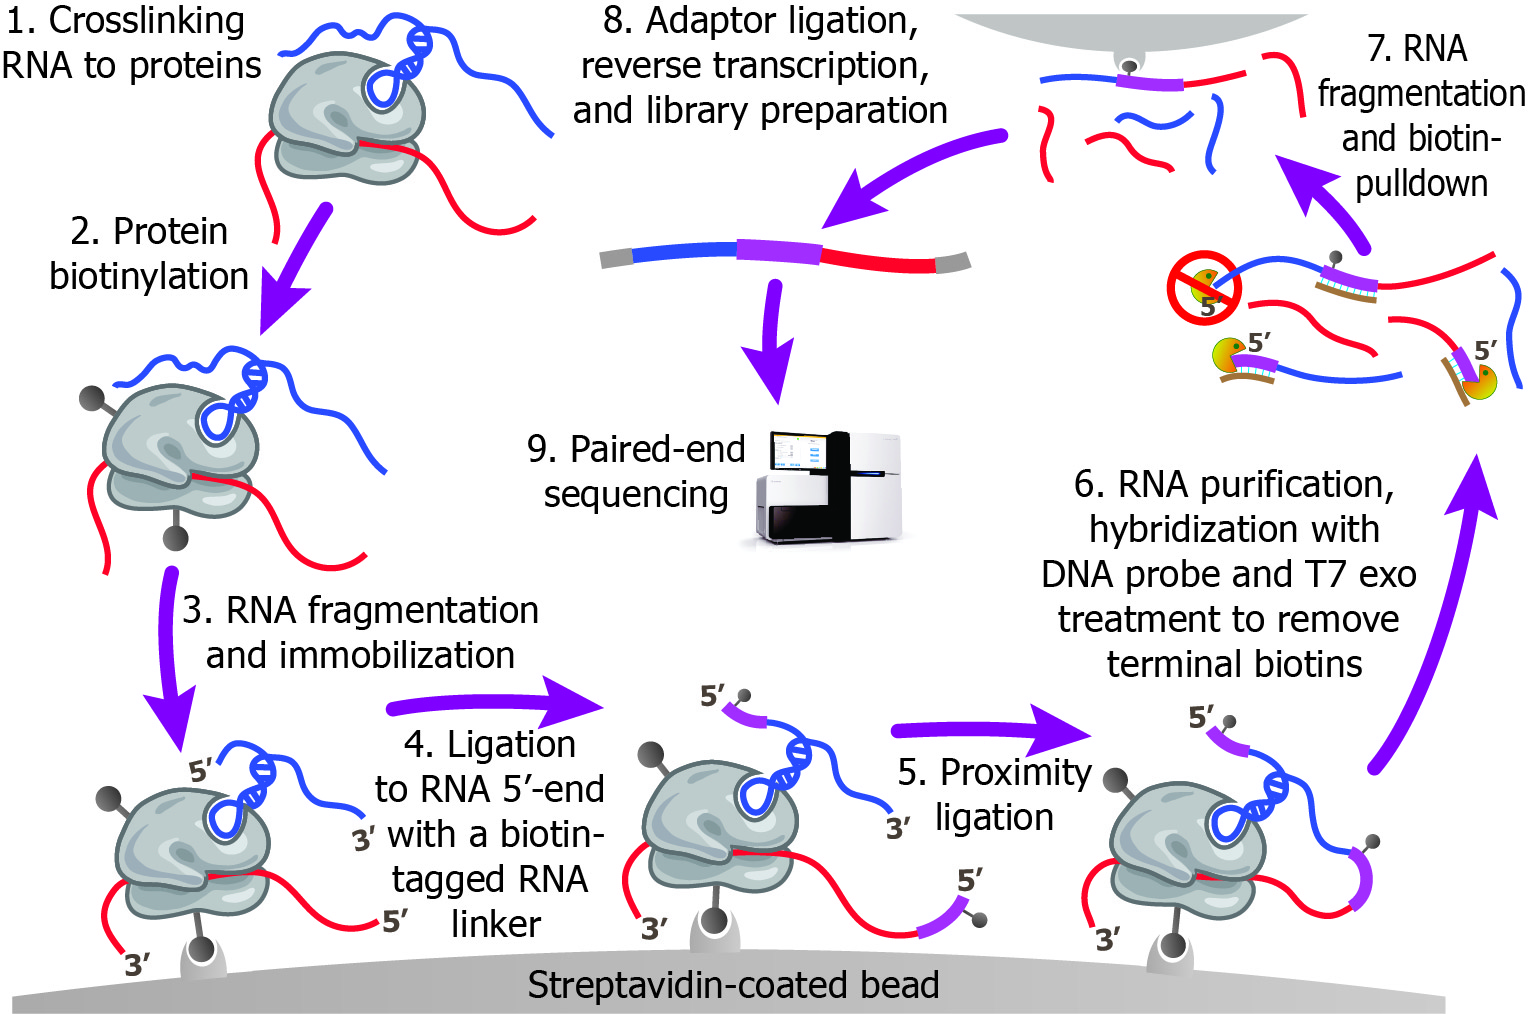
\includegraphics{exp.jpg}\hfill}

Below is a illustration for the experimental design of this new technology. This procedure crosslinks RNAs with their bound proteins, and ligates the RNAs co-bound by the same protein into a chimeric RNA. The chimeric RNA is interspersed by a predesigned biotinylated RNA linker, in the form of RNA1-Linker-RNA2. These linker-containing chimeric RNAs are selected by streptavidin and then subjected to pair-end sequencing

The RNA Hi-C method offers several advantages for mapping RNA-RNA interactions. First, the one-to-one pairing of interacting RNAs is experimentally captured. Second, by using the biotinylated linker as a selection marker, it circumvents the requirement for either a protein-specific antibody or expressing a tagged protein, allowing for an as unbiased mapping of the entire RNA interactome as possible. Third, false positive interactions, produced by ligation of random RNAs that happened to be proximal in space, are minimized by performing RNA ligation on streptavidin beads in a dilute condition. Fourth, the predesigned RNA linker provides a clear boundary to split any sequencing read that spans across the ligation spot, thus avoids ambiguities in mapping the sequencing reads. Fifth, RNA Hi-C directly analyzes the endogenous cellular condition without introducing any exogenous nucleotides or protein-coding genes before crosslinking. Sixth, potential PCR amplification biases were removed by attaching a random 6nt barcode to each chimeric RNA before PCR amplification, where the completely overlapping sequencing reads with identical barcodes are counted only once.


\strong{See also:}


Offline documentation.

Download a copy of RNA-Hi-C-tools documentation:
\begin{itemize}
\item {} 
\href{http://systemsbio.ucsd.edu/RNA-Hi-C/\_sources/Stitch-seq-tools.pdf}{PDF}

\item {} 
\href{https://media.readthedocs.org/epub/stitch-seq-tools/latest/stitch-seq-tools.epub}{Epub}

\end{itemize}




\section{Installation}
\label{RNA-Hi-C-tools:installation}

\subsection{step 1: Install the dependent prerequisites:}
\label{RNA-Hi-C-tools:step-1-install-the-dependent-prerequisites}\begin{enumerate}
\item {} 
Python libraries {[}for python 2.x{]}:

\end{enumerate}
\begin{itemize}
\item {} 
\href{http://biopython.org/wiki/Main\_Page}{Biopython}

\item {} 
\href{https://code.google.com/p/pysam/}{Pysam}

\item {} 
\href{http://bam2xwiki.appspot.com/Welcome}{BAM2X}

\item {} 
\href{http://www.numpy.org/}{Numpy}, \href{http://www.scipy.org/scipylib/index.html}{Scipy}

\item {} 
\href{http://www.parallelpython.com/}{Parallel python} (Only for \code{Select\_strongInteraction\_pp.py})

\end{itemize}
\begin{enumerate}
\setcounter{enumi}{1}
\item {} 
The \href{http://www.boost.org/doc/libs/1\_54\_0/libs/python/doc/index.html}{Boost.Python} C++ library

\item {} 
Other softwares needed:

\end{enumerate}
\begin{itemize}
\item {} 
\href{http://bowtie-bio.sourceforge.net/index.shtml}{Bowtie} (or Bowtie 2 if you set Bowtie2 option in \code{Stitch-seq\_Aligner.py})

\item {} 
\href{http://samtools.sourceforge.net/}{samtools}

\item {} 
\href{ftp://ftp.ncbi.nlm.nih.gov/blast/executables/blast+/LATEST/}{NCBI blast+} (use blastn)

\end{itemize}


\subsection{Step 2: Download the package}
\label{RNA-Hi-C-tools:step-2-download-the-package}
Clone the package from GitHub:

\begin{Verbatim}[commandchars=\\\{\}]
git clone http://github.com/yu68/RNA-Hi-C.git
\end{Verbatim}


\subsection{Step 3: Add library source to your python path}
\label{RNA-Hi-C-tools:step-3-add-library-source-to-your-python-path}
Add these lines into your \textasciitilde{}/.bash\_profile or \textasciitilde{}/.profile

\begin{Verbatim}[commandchars=\\\{\}]
Location="/path/of/RNA-Hi-C-tools" \# change accordingly
export PYTHONPATH="\$Location/src:\$PYTHONPATH"
export PATH="\$PATH:\$Location/bin"
Loc\_lib="/path/of/boost\_1\_xx\_0/lib/"  \# change accordingly
export LD\_LIBRARY\_PATH="\$Loc\_lib:\$LD\_LIBRARY\_PATH"
\end{Verbatim}


\section{Support}
\label{RNA-Hi-C-tools:support}
For issues related to the use of RNA-Hi-C-tools, or if you want to \textbf{report a bug or request a feature}, please contact Pengfei Yu \textless{}p3yu at ucsd dot edu\textgreater{}


\chapter{Analysis pipeline}
\label{Analysis_pipeline:analysis-pipeline}\label{Analysis_pipeline::doc}

\section{Overview}
\label{Analysis_pipeline:overview}
The next generation DNA sequencing based technology utilize RNA proximity ligation to transfrom RNA-RNA interactions into chimeric DNAs. Through sequencing and mapping these chimeric DNAs, it is able to achieve high-throughput mapping of nearly entire interaction networks. RNA linkers were introduced to mark the junction of the ligation and help to split the chimeric RNAs into two interacting RNAs.
This bioinformatic pipeline is trying to obtain the strong interactions from raw fastq sequencing data. The major steps are:
\begin{itemize}
\item {} 
{\hyperref[Analysis_pipeline:step1]{\emph{Step 1: Remove PCR duplicates.}}}

\item {} 
{\hyperref[Analysis_pipeline:step2]{\emph{Step 2: Split library based on barcode.txt.}}}

\item {} 
{\hyperref[Analysis_pipeline:step3]{\emph{Step 3: Recover fragments for each library.}}}

\item {} 
{\hyperref[Analysis_pipeline:step4]{\emph{Step 4: Split partners and classify different types of fragments.}}}

\item {} 
{\hyperref[Analysis_pipeline:step5]{\emph{Step 5: Align both parts of ``Paired'' fragment to the genome.}}}

\item {} 
{\hyperref[Analysis_pipeline:step6]{\emph{Step 6: Determine strong interactions.}}}

\item {} 
{\hyperref[Analysis_pipeline:step7]{\emph{Step 7: Visualization of interactions and coverages.}}}

\end{itemize}

Other functions:
\begin{enumerate}
\item {} 
{\hyperref[Analysis_pipeline:rna-types]{\emph{Determine the RNA types of different parts within fragments.}}}

\item {} 
{\hyperref[Analysis_pipeline:find-linker]{\emph{Find linker sequences within the library.}}}

\item {} 
{\hyperref[Analysis_pipeline:intersection]{\emph{Find intersections between two different interaction sets based on genomic locations}}}

\item {} 
{\hyperref[Analysis_pipeline:intersectiongene]{\emph{Find intersections between two different interaction sets based on annotation}}}

\item {} 
{\hyperref[Analysis_pipeline:structure]{\emph{RNA structure prediction by adding digestion site information}}}

\end{enumerate}


\section{Pipeline}
\label{Analysis_pipeline:pipeline}

\subsection{Step 1: Remove PCR duplicates.}
\label{Analysis_pipeline:step-1-remove-pcr-duplicates}\label{Analysis_pipeline:step1}
\index{remove\_dup\_PE.py}
Starting from the raw pair-end sequencing data, PCR duplicates should be removed as the first step if both the 10nt random indexes and the remaining sequences are exactly the same for two pairs. It is achieved by \code{remove\_dup\_PE.py}

\begin{Verbatim}[commandchars=\\\{\}]
usage: remove\_dup\_PE.py [-h] reads1 reads2

Remove duplicated reads which have same sequences for both forward and reverse
reads. Choose the one appears first.

positional arguments:
  reads1      forward input fastq/fasta file
  reads2      reverse input fastq/fasta file

optional arguments:
  -h, --help  show this help message and exit

Library dependency: Bio, itertools
\end{Verbatim}

The program will generate two fastq/fasta files after removind PCR duplicates and report how many read pairs has been removed. The output are prefixed with `Rm\_dupPE'

\begin{notice}{note}{Note:}
One pair is considered as a PCR duplicate only when the sequences of both two ends (including the 10nt random index) are the exactly same as any of other pairs.
\end{notice}


\subsection{Step 2: Split library based on barcode.txt.}
\label{Analysis_pipeline:step-2-split-library-based-on-barcode-txt}\label{Analysis_pipeline:step2}
\index{split\_library\_pairend.py}
After removing PCR duplicates, the libraries from different samples are separated based on 4nt barcodes in the middle of random indexes (``RRRBBBBRRR''; R: random, B: barcode). It is implemented by \code{split\_library\_pairend.py}

\begin{Verbatim}[commandchars=\\\{\}]
usage: split\_library\_pairend.py [-h] [-f \textbar{} -q] [-v] [-b BARCODE]
                                [-r RANGE [RANGE ...]] [-t] [-m MAX\_SCORE]
                                input1 input2

Example: split\_library\_pairend.py -q Rm\_dupPE\_example.F1.fastq
         Rm\_dupPE\_example.R1.fastq -b barcode.txt

positional arguments:
  input1                input fastq/fasta file 1 for pairend data (contain
                        barcodes)
  input2                input fastq/fasta file 2 for pairend data

optional arguments:
  -h, --help            show this help message and exit
  -f, --fasta           add this option for fasta input file
  -q, --fastq           add this option for fastq input file
  -v, --version         show program's version number and exit
  -b BARCODE, --barcode BARCODE
                        barcode file
  -r RANGE [RANGE ...], --range RANGE [RANGE ...]
                        set range for barcode location within reads,default is
                        full read
  -t, --trim            trim sequence of 10nt index
  -m MAX\_SCORE, --max\_score MAX\_SCORE
                        max(mismatch+indel) allowed for barcode match,
                        otherwise move reads into 'unassigned' file
                        default: 2.

Library dependency: Bio
\end{Verbatim}

Here is a example for barcode.txt

\begin{Verbatim}[commandchars=\\\{\}]
\PYG{n}{ACCT}
\PYG{n}{CCGG}
\PYG{n}{GGCG}
\end{Verbatim}

The output of this script are several pairs of fastq/fasta files prefixed with the 4nt barcode sequences, together with another pair of fastq/fasta files prefixed with `unassigned'.

For example, if the input fastq/fasta files are \code{Rm\_dupPE\_example.F1.fastq} and \code{Rm\_dupPE\_example.R1.fastq}, and the barcode file is the same as above, then the output files are:
\begin{itemize}
\item {} 
ACCT\_Rm\_dupPE\_example.F1.fastq

\item {} 
ACCT\_Rm\_dupPE\_example.R1.fastq

\item {} 
CCGG\_Rm\_dupPE\_example.F1.fastq

\item {} 
CCGG\_Rm\_dupPE\_example.R1.fastq

\item {} 
GGCG\_Rm\_dupPE\_example.F1.fastq

\item {} 
GGCG\_Rm\_dupPE\_example.R1.fastq

\item {} 
unassigned\_Rm\_dupPE\_example.F1.fastq

\item {} 
unassigned\_Rm\_dupPE\_example.R1.fastq

\end{itemize}


\subsection{Step 3: Recover fragments for each library.}
\label{Analysis_pipeline:step-3-recover-fragments-for-each-library}\label{Analysis_pipeline:step3}
\index{recoverFragment}
\textbf{After splitting the libraries, the later steps from here (Step 3-7) need to be executed parallelly for each sample.}

In this step, we are trying to recover the fragments based on local alignment. The fragments are classifed as several different types as shown in the figure below. The flow chart is also clarified at the top.

{\hfill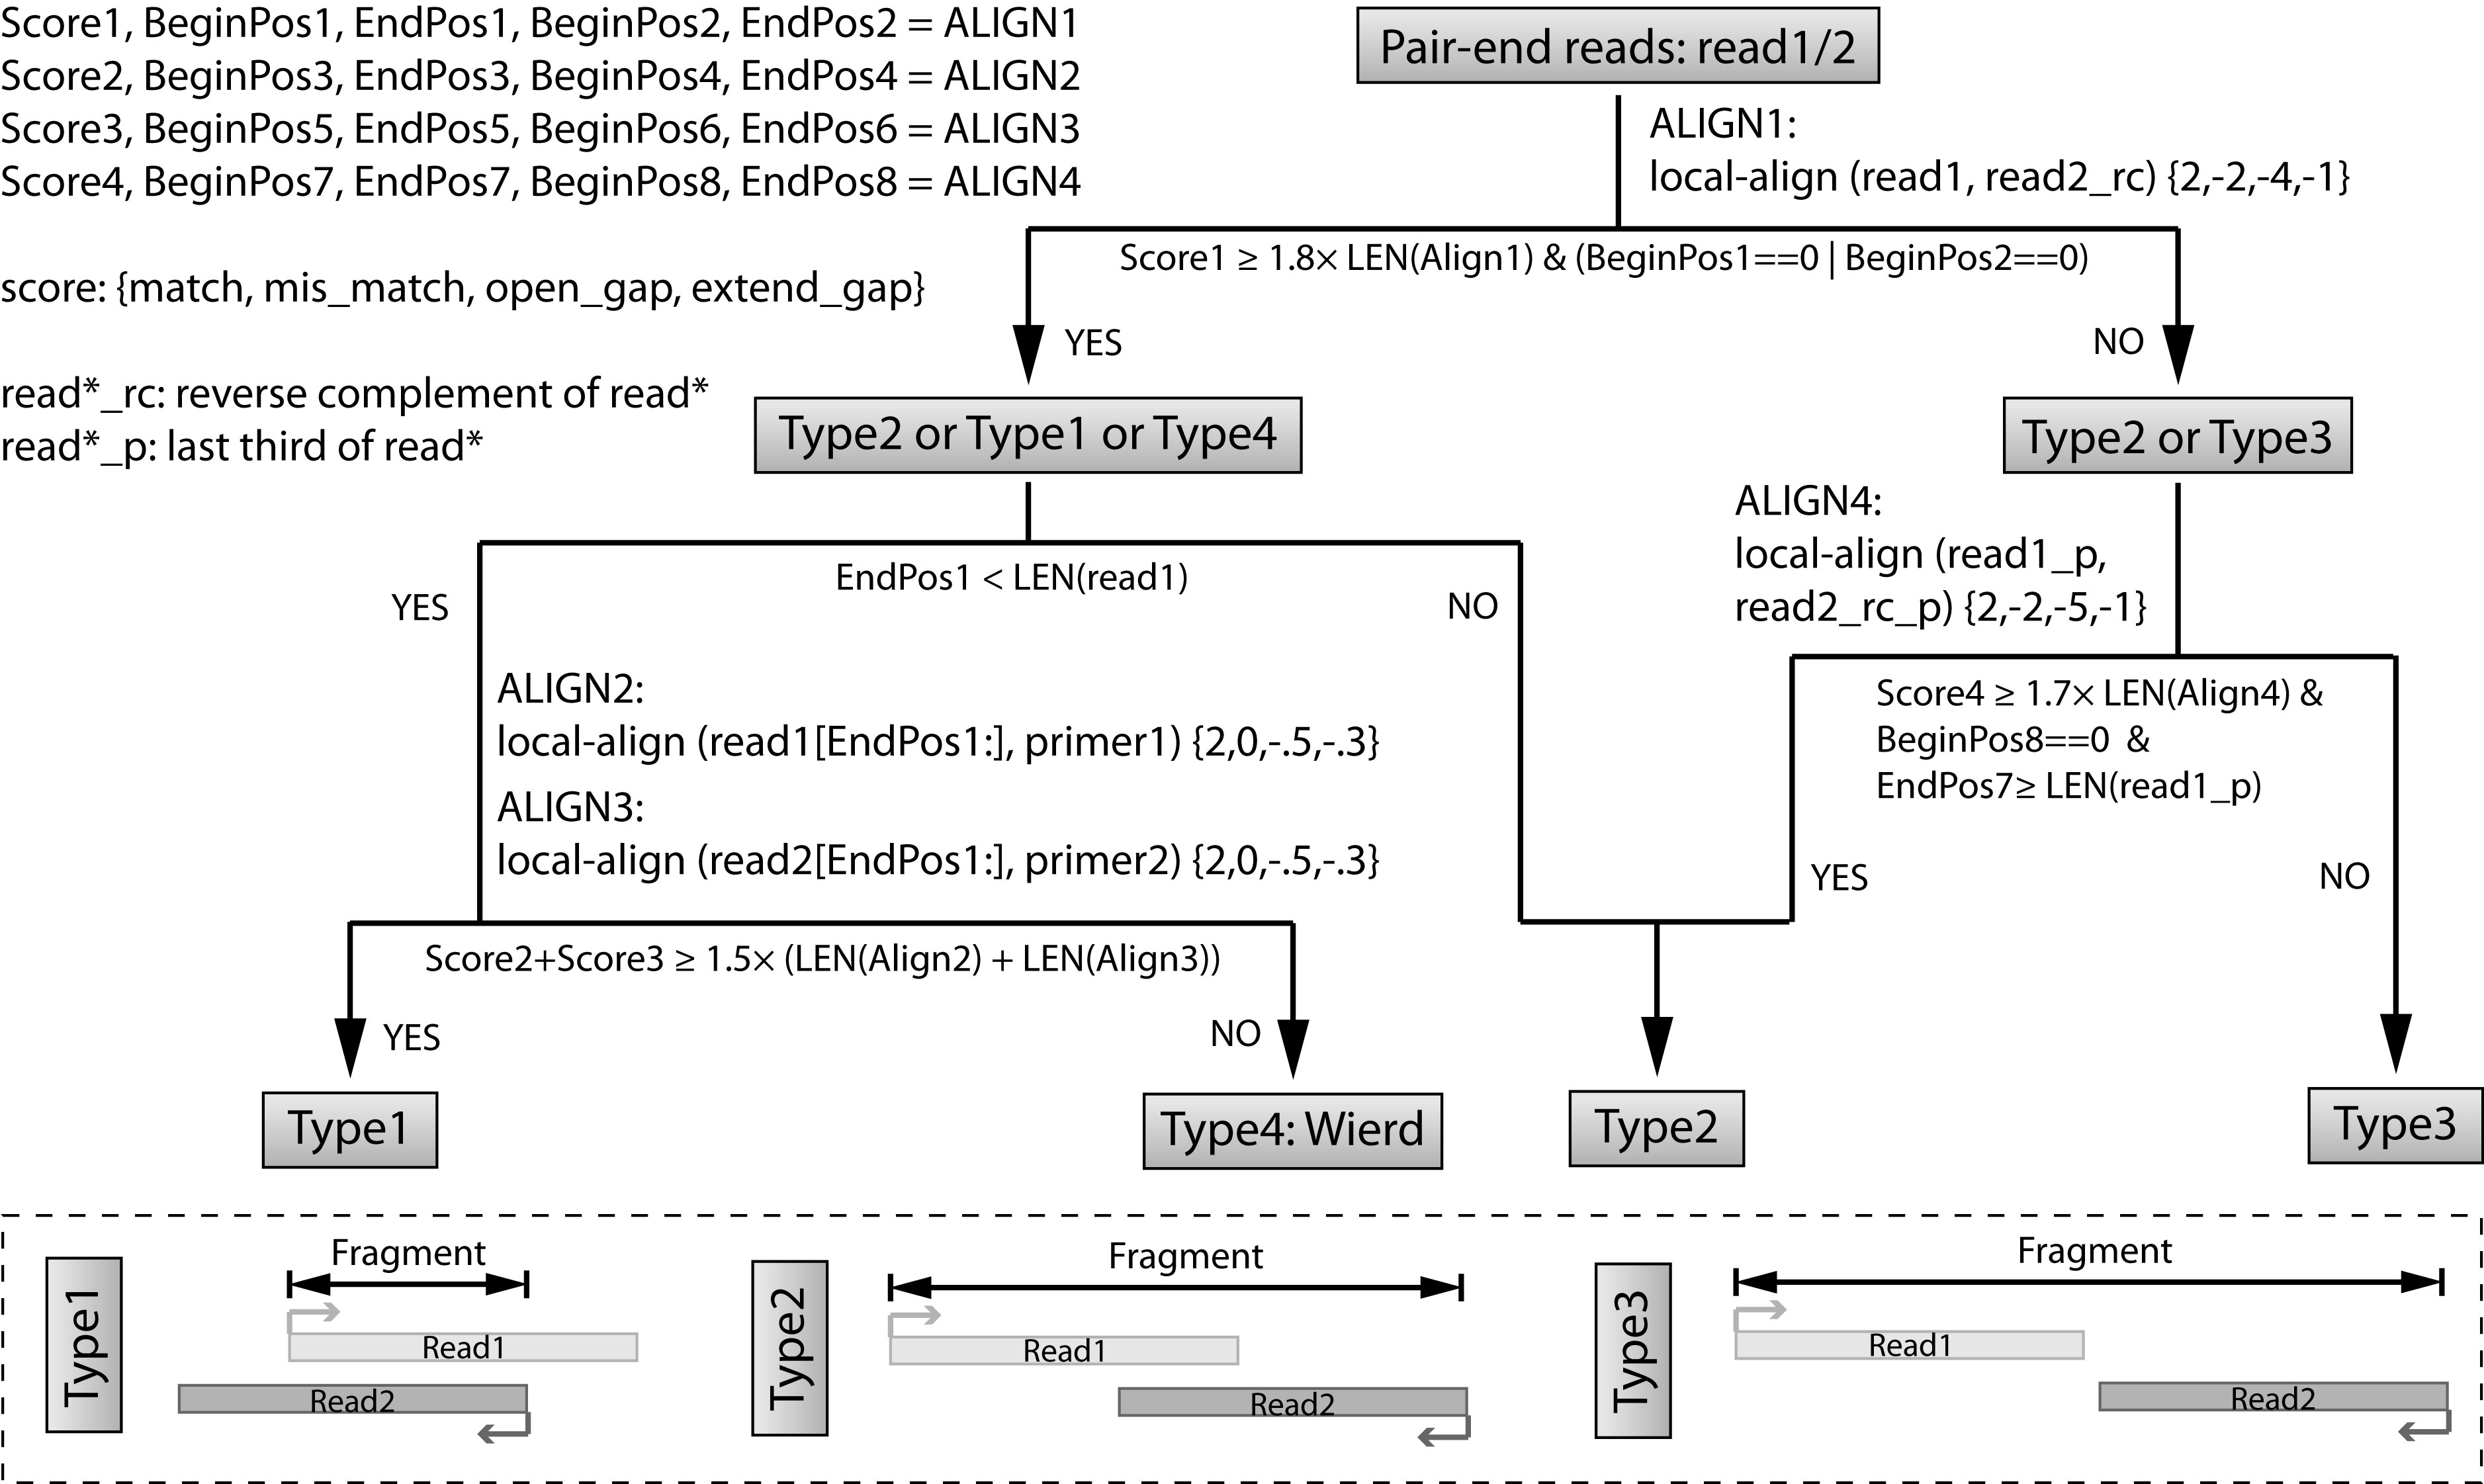
\includegraphics{workflow_for_recoverFragment.jpg}\hfill}

We will use a complied program \code{recoverFragment} to do that

\begin{Verbatim}[commandchars=\\\{\}]
recoverFragment - recover fragment into 4 different categories from pair-end seq data
=====================================================================================

SYNOPSIS

DESCRIPTION
    -h, --help
          Displays this help message.
    --version
          Display version information
    -I, --inputs STR
          input of forward and reverse fastq file, path of two files separated by SPACE
    -p, --primer STR
          fasta file contianing two primer sequences
    -v, --verbose
          print alignment information for each alignment

EXAMPLES
    recoverFragment -I read\_1.fastq read\_2.fastq -p primer.fasta
          store fragment using fasta/fastq into 4 output files
          'short\_*', 'long\_*','evenlong\_*','wierd\_*'

VERSION
    recoverFragment version: 0.1
    Last update August 2013
\end{Verbatim}


\subsection{Step 4: Split partners and classify different types of fragments.}
\label{Analysis_pipeline:step4}\label{Analysis_pipeline:step-4-split-partners-and-classify-different-types-of-fragments}
\index{split\_partner.py}
When we recovered the fragments, the next we are goting to do is to find RNA1 and RNA2 that are seprarated by the linkers, and from here, we will be able to classify the fragments into different types: ``IndexOnly'', ``NoLinker'', ``LinkerOnly'', ``BackOnly'', ``FrontOnly'', ``Paired''. (see the figure below).

{\hfill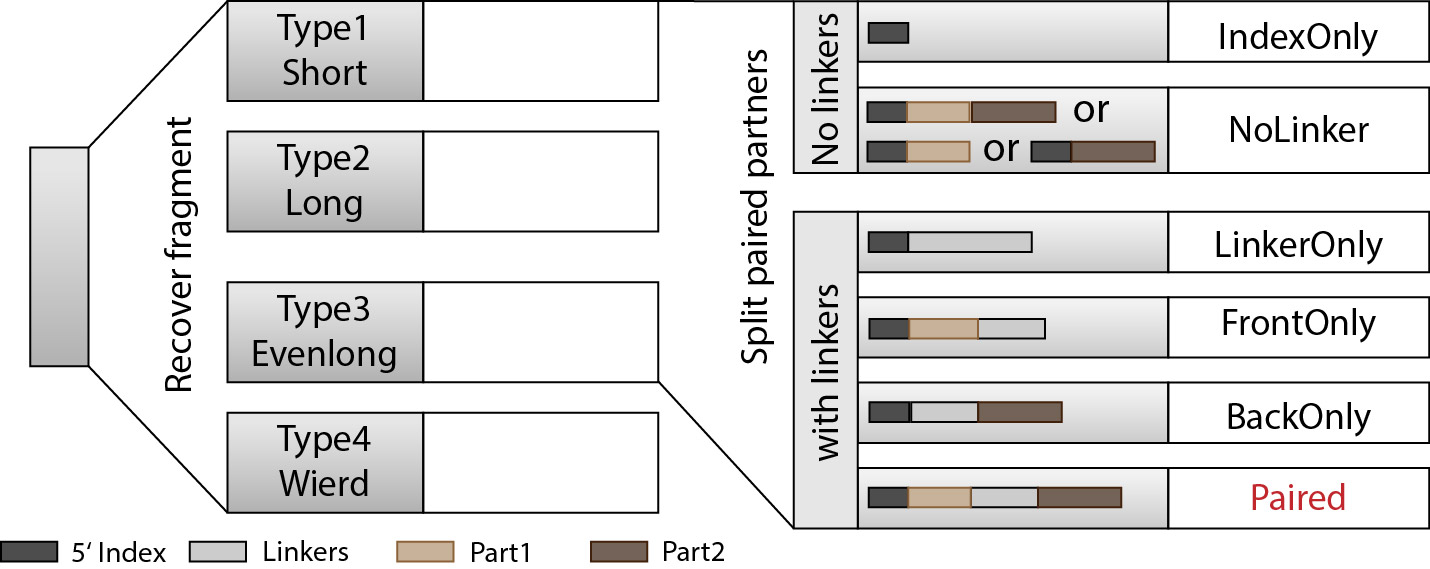
\includegraphics{summary.jpg}\hfill}

This will be done by \code{split\_partner.py}

\begin{Verbatim}[commandchars=\\\{\}]
usage: split\_partner.py [-h] [-e EVALUE] [--linker\_db LINKER\_DB]
                        [--blast\_path BLAST\_PATH] [-o OUTPUT] [-t TRIM]
                        [-b BATCH] [-l LENGTH]
                        input type3\_1 type3\_2

DESCRIPTION: Run BLAST, find linker sequences and split two parts connected by
linkers

positional arguments:
  input                 the input fasta file containing fragment sequences of
                        type1 and type2
  type3\_1               read\_1 for evenlong (type3) fastq file
  type3\_2               read\_2 for evenlong (type3) fastq file

optional arguments:
  -h, --help            show this help message and exit
  -e EVALUE, --evalue EVALUE
                        cutoff evalues, only choose alignment with evalue less
                        than this cutoffs (default: 1e-5).
  --linker\_db LINKER\_DB
                        BLAST database of linker sequences
  --blast\_path BLAST\_PATH
                        path for the local blast program
  -o OUTPUT, --output OUTPUT
                        output file containing sequences of two sepatated
                        parts
  -t TRIM, --trim TRIM  trim off the first this number of nt as index,
                        default:10
  -b BATCH, --batch BATCH
                        batch this number of fragments for BLAST at a time.
                        default: 200000
  -r, --release         set to allow released criterion for Paired fragment in
                        Type 3, include those ones with no linker in two reads
  -l LENGTH, --length LENGTH
                        shortest length to be considered for each part of the
                        pair, default: 15

Library dependency: Bio, itertools
\end{Verbatim}

\begin{notice}{note}{Note:}
New option added in version 0.3.1, which could allow two different strategies for selection of ``Paired'' fragments from the Type3 fragments. The \code{-{-}release} option will allow a read pair to be called as ``Paired'' fragment even when the linker are not detected in both reads.
\end{notice}

The linker fasta file contain sequences of all linkers

\begin{Verbatim}[commandchars=\\\{\}]
\textgreater{}L1
CTAGTAGCCCATGCAATGCGAGGA
\textgreater{}L2
AGGAGCGTAACGTACCCGATGATC
\end{Verbatim}

The output fasta files will be the input file name with different prefix (``NoLinker'', ``LinkerOnly'', ``BackOnly'', ``FrontOnly'', ``Paired'') for different types. The other output file specified by \code{-o} contains information of aligned linker sequences for each Type1/2 fragment.

For example, if the commend is

\begin{Verbatim}[commandchars=\\\{\}]
split\_partner.py fragment\_ACCT.fasta evenlong\_ACCTRm\_dupPE\_stitch\_seq\_1.fastq
    evenlong\_ACCTRm\_dupPE\_stitch\_seq\_2.fastq
    -o fragment\_ACCT\_detail.txt --linker\_db linker.fa
\end{Verbatim}
\begin{description}
\item[{Then, the output files will be:}] \leavevmode\begin{itemize}
\item {} 
backOnly\_fragment\_ACCT.fasta

\item {} 
NoLinker\_fragment\_ACCT.fasta

\item {} 
frontOnly\_fragment\_ACCT.fasta

\item {} 
Paired1\_fragment\_ACCT.fasta

\item {} 
Paired2\_fragment\_ACCT.fasta

\item {} 
fragment\_ACCT\_detail.txt

\end{itemize}

\end{description}

The format of the last output file \code{fragment\_ACCT\_detail.txt} will be ``Name \textbar{} linker\_num \textbar{} linker\_loc \textbar{} Type \textbar{} linker\_order''. Here are two examples:

\begin{Verbatim}[commandchars=\\\{\}]
HWI-ST1001:238:H0NYEADXX:1:1101:10221:1918      L1:2;L2:1  19,41;42,67;68,97       None    L2;L1;L1
HWI-ST1001:238:H0NYEADXX:1:1101:4620:2609       L1:2 28,46;47,79     Paired  L1;L1
\end{Verbatim}

In the \textbf{first} fragment, there are three regions can be aligned to linkers, 2 for L1 and 1 for L2, the order is L2, L1, L1. And they are aligned in region {[}19,41{]}, {[}42,67{]}, {[}68,97{]} of the fragment. ``None'' means this fragment is either `LinkerOnly' or `IndexOnly' (in this case it is `LinkerOnly'). This fragment won't be written to any of the output fasta files.

In the \textbf{second} fragment, two regions can be aligned to linkers, and they are both aligned to L1. The two regions are in {[}28,46{]}, {[}47,79{]} of the fragment. the fragment is ``Paired'' because on both two sides flanking the linker aligned regions, the length is larger than 15nt. The left part will be writen in \code{Paired1\_fragment\_ACCT.fasta} and the right part in \code{Paired2\_fragment\_ACCT.fasta}


\subsection{Step 5: Align both parts of ``Paired'' fragment to the genome.}
\label{Analysis_pipeline:step-5-align-both-parts-of-paired-fragment-to-the-genome}\label{Analysis_pipeline:step5}
\index{Stitch-seq\_Aligner.py}
In this step, we will use the Paired1* and Paired2* fasta files output from the previous step. The sequences of part1 and part2 are aligned to the mouse genome mm9 with Bowtie and the pairs with both part1 and part2 mappable are selected as output. We also annotate the RNA types of each part in this step.
All of these are implemented using script \code{Stitch-seq\_Aligner.py}.

\begin{Verbatim}[commandchars=\\\{\}]
usage: Stitch-seq\_Aligner.py [-h] [-s samtool\_path] [-a ANNOTATION]
                             [-A DB\_DETAIL]
                             miRNA\_reads mRNA\_reads bowtie\_path miRNA\_ref
                             mRNA\_ref

Align miRNA-mRNA pairs for Stitch-seq. print the alignable miRNA-mRNA pairs
with coordinates

positional arguments:
  part1\_reads           paired RNA1 fasta file
  part2\_reads           paired RNA2 fasta file
  bowtie\_path           path for the bowtie program
  part1\_ref             reference genomic seq for RNA1
  part2\_ref             reference genomic seq for RNA2

optional arguments:
  -h, --help            show this help message and exit
  -b, --bowtie2         set to use bowtie2 (--sensitive-local) for alignment,
                        need to change reference index and bowtie\_path
  -u, --unique          set to only allow unique alignment
  -s samtool\_path, --samtool\_path samtool\_path
                        path for the samtool program
  -a ANNOTATION, --annotation ANNOTATION
                        If specified, include the RNA type annotation for each
                        aligned pair, need to give bed annotation RNA file
  -A DB\_DETAIL, --annotationGenebed DB\_DETAIL
                        annotation bed12 file for lincRNA and mRNA with intron
                        and exon

Library dependency: Bio, pysam, itertools
\end{Verbatim}

An annotation file for different types of RNAs in mm9 genome (bed format, `all\_RNAs-rRNA\_repeat.txt.gz') was included in Data folder. The annotation bed12 file for lincRNA and mRNA (`Ensembl\_mm9.genebed.gz') was also included in Data folder. One can use the option \code{-a ../Data/all\_RNAs-rRNA\_repeat.txt.gz -A ../Data/Ensembl\_mm9.genebed.gz} for annotation.

Here is a example:

\begin{Verbatim}[commandchars=\\\{\}]
Stitch-seq\_Aligner.py Paired1\_fragment\_ACCT.fasta Paired2\_fragment\_ACCT.fasta
    \textasciitilde{}/Software/bowtie-0.12.7/bowtie mm9 mm9 -s samtools
    -a ../Data/all\_RNAs-rRNA\_repeat.txt.gz -A ../Data/Ensembl\_mm9.genebed.gz
    \textgreater{} ACCT\_fragment\_paired\_align.txt
\end{Verbatim}

The format for the output file \code{ACCT\_fragment\_paired\_align.txt} will be:
\begin{quote}

\begin{tabulary}{\linewidth}{|L|L|}
\hline
\textsf{\relax 
Column \footnote{
column 10-17 are the same as column 1-8 except they are for RNA2 instead of RNA1.
}
} & \textsf{\relax 
Description
}\\
\hline
1
 & 
chromosome name of RNA1
\\

2,3
 & 
start/end position of RNA1
\\

4
 & 
strand information of RNA1
\\

5
 & 
sequence of RNA1
\\

6
 & 
RNA type for RNA1
\\

7
 & 
RNA name for RNA1
\\

8
 & 
RNA subtype \footnote{
subtype can be intron/exon/utr5/utr3 for lincRNA and mRNA (protein-coding), `.' for others
} for RNA1
\\

9
 & 
name of the pair
\\
\hline\end{tabulary}

\end{quote}

\begin{notice}{note}{Note:}
Bowtie2 (``--sensitive-local'' mode) option is added in version 0.3.1 for the user to choose, the \code{reference index} and \code{bowtie\_path} need to be changed accordingly if you use bowtie2 instead of bowtie. User can also choose unique aligned reads or not by setting \code{-{-}unique} option.
\end{notice}


\subsection{Step 6: Determine strong interactions.}
\label{Analysis_pipeline:step6}\label{Analysis_pipeline:step-6-determine-strong-interactions}
\index{Select\_strongInteraction\_pp.py}
In this step, we will generate clusters with high coverage separately for all RNA1 (R1) an RNA2 (R2) segments. Then based on the pairing information, we count the interactions between clusters from RNA1 and RNA2. For each interaction between clusters in RNA1 and RNA2, a p-value can be generated based on hypergeometric distribution. Given the p-values of all interactions, we could adjust the p-values controlled by False Discovery Rate (FDR, Benjamini-Hochberg procedure). The strong interactions can be selected by applying a FDR cutoff from adjusted p-values. (See figure below)

{\hfill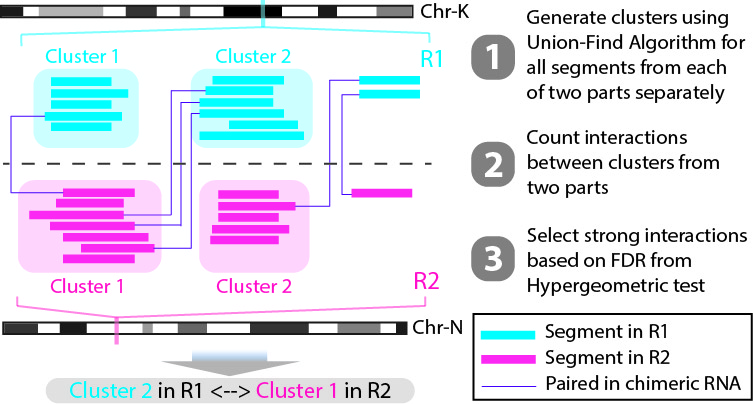
\includegraphics{Find_strong_interaction.jpg}\hfill}

We will use the script \code{Select\_strongInteraction\_pp.py}, parallel computing are implemented for clustering parallelly on different chromosomes:

\begin{Verbatim}[commandchars=\\\{\}]
usage: Select\_strongInteraction\_pp.py [-h] -i INPUT [-M MIN\_CLUSTERS]
                                      [-m MIN\_INTERACTION] [-p P\_VALUE]
                                      [-o OUTPUT] [-P PARALLEL] [-F]

find strong interactions from paired genomic location data

optional arguments:
  -h, --help            show this help message and exit
  -i INPUT, --input INPUT
                        input file which is the output file of Stitch-seq-
                        Aligner.py
  -M MIN\_CLUSTERS, --min\_clusterS MIN\_CLUSTERS
                        minimum number of segments allowed in each cluster,
                        default:5
  -m MIN\_INTERACTION, --min\_interaction MIN\_INTERACTION
                        minimum number of interactions to support a strong
                        interaction, default:3
  -p P\_VALUE, --p\_value P\_VALUE
                        the p-value based on hypergeometric distribution to
                        call strong interactions, default: 0.05
  -o OUTPUT, --output OUTPUT
                        specify output file
  -P PARALLEL, --parallel PARALLEL
                        number of workers for parallel computing, default: 5
  -F, --FDR             Compute FDR if specified

need Scipy for hypergeometric distribution
\end{Verbatim}

The input of the script is the output of Step 5 (\code{ACCT\_fragment\_paired\_align.txt} in the example). ``annotated\_bed'' class is utilized in this script.

Here is a example:

\begin{Verbatim}[commandchars=\\\{\}]
Select\_strongInteraction.py -i ACCT\_fragment\_paired\_align.txt -o ACCT\_interaction\_clusters.txt
\end{Verbatim}

The column description for output file \code{ACCT\_interaction\_clusters.txt} is:
\begin{quote}

\begin{tabulary}{\linewidth}{|L|L|}
\hline
\textsf{\relax 
Column
} & \textsf{\relax 
Description
}\\
\hline
1
 & 
chromosome name of cluster in RNA1
\\

2,3
 & 
start/end position of cluster in RNA1
\\

4
 & 
RNA type for cluster in RNA1
\\

5
 & 
RNA name for cluster in RNA1
\\

6
 & 
RNA subtype for cluster in RNA1
\\

7
 & 
\# of counts for cluster in RNA1
\\

8-14
 & 
Same as 1-7, but for cluster in RNA2
\\

15
 & 
\# of interactions between these two clusters
\\

16
 & 
log(p-value) of the hypergeometric testing
\\
\hline\end{tabulary}

\end{quote}


\subsection{Step 7: Visualization of interactions and coverages.}
\label{Analysis_pipeline:step7}\label{Analysis_pipeline:step-7-visualization-of-interactions-and-coverages}
There are two ways of visulization provided ( LOCAL and GLOBAL ):
\begin{itemize}
\item {} 
{\hyperref[Visualization:visualizationlocal]{\emph{Visualization of local interactions}}}.

\item {} 
{\hyperref[Visualization:visualizationglobal]{\emph{Visualization of global interactome}}}.

\end{itemize}


\section{Other functions}
\label{Analysis_pipeline:other-functions}

\subsection{Determine the RNA types of different parts within fragments.}
\label{Analysis_pipeline:rna-types}\label{Analysis_pipeline:determine-the-rna-types-of-different-parts-within-fragments}

\subsection{Find linker sequences within the library.}
\label{Analysis_pipeline:find-linker-sequences-within-the-library}\label{Analysis_pipeline:find-linker}

\subsection{Find intersections between two different interaction sets based on genomic locations}
\label{Analysis_pipeline:find-intersections-between-two-different-interaction-sets-based-on-genomic-locations}\label{Analysis_pipeline:intersection}
\index{intersectInteraction.py}
The script tool \code{intersectInteraction.py} could be used to identify overlap of interactions between two interaction set from independent experiments based on genomic locations (two replicates or two different samples)

\begin{Verbatim}[commandchars=\\\{\}]
usage: intersectInteraction.py [-h] -a FILEA -b FILEB [-s START] [-n NBASE]
                               [-o OUTPUT] [-c]

find intersections (overlaps) between two interaction sets

optional arguments:
  -h, --help            show this help message and exit
  -a FILEA, --filea FILEA
                        file for interaction set a
  -b FILEB, --fileb FILEB
                        file for interaction set b
  -s START, --start START
                        start column number of the second part in each
                        interaction (0-based), default:7
  -n NBASE, --nbase NBASE
                        number of overlapped nucleotides for each part of
                      interactions to call intersections, default: 1
  -o OUTPUT, --output OUTPUT
                        specify output file
  -p, --pvalue          calculate p-values based on 100times permutations

require 'random'\&'numpy'\&'scipy' module if set '-p'
\end{Verbatim}

if ``-p'' option is set, then the program will do permutation for 100 times by shuffling the two partners of interactions in set a. A p-value will be calculate based on permutation distribution.


\subsection{Find intersections between two different interaction sets based on annotation}
\label{Analysis_pipeline:intersectiongene}\label{Analysis_pipeline:find-intersections-between-two-different-interaction-sets-based-on-annotation}
\index{intersectInteraction\_genePair.R}
The script tool \code{intersectInteraction\_genePair.R} could be used to identify overlap of interactions between two interaction set from independent experiments based on the RNA annotations (two replicates or two different samples)

\begin{Verbatim}[commandchars=\\\{\}]
usage: intersectInteraction\_genePair.R [-h] [-n NUM [NUM ...]] [-p] [-r]
                                       [-o OUTPUT]
                                       interactionA interactionB

Call intersections based on gene pairs

positional arguments:
  interactionA          the interaction file a,[required]
  interactionB          the interaction file b,[required]

optional arguments:
  -h, --help            show this help message and exit
  -n NUM [NUM ...], --num NUM [NUM ...]
                        Column numbers for the gene name in two part,[default:
                        [5, 12]]
  -p, --pvalue          set to do 100 permutations for p-value of overlap
  -r, --release         set to only require match of chromosome and RNA name,
                        but not subtype
  -o OUTPUT, --output OUTPUT
                        output intersection file name, pairs in A that overlap
                        with B, [default: intersect.txt]
\end{Verbatim}

if ``-p'' option is set, then the program will do permutation for 100 times by shuffling the two partners of interactions in both set a and set b. A p-value will be calculate based on permutation distribution.


\subsection{RNA structure prediction by adding digestion site information}
\label{Analysis_pipeline:rna-structure-prediction-by-adding-digestion-site-information}\label{Analysis_pipeline:structure}
\index{RNA\_structure\_prediction.py}
The script will take selfligated chimeric fragments from given snoRNA (ID) and predict secondary structures with and without constraints of digested single strand sites. It is also able to compare the known structure in dot format if the known structure is available and specified by ``-a''. The script needs RNAStructure software for structure prediction (``-R'') and  and VARNA command line tool for visualization (``-v'').

\begin{Verbatim}[commandchars=\\\{\}]
usage: RNA\_structure\_prediction.py [-h] [-g GENOMEFA] [-R RNASTRUCTUREEXE]
                                 [-a ACCEPTDOT] [-o OUTPUT]
                                 [-s samtool\_path] [-v VARNA]
                                 [-c COLORMAPSTYLE]
                                 ID linkedPair

plot RNA structure with distribution of digested end, refine structure with
loc of digested end

positional arguments:
  ID                    Ensembl gene ID of RNA
  linkedPair            file for information of linked pairs, which is output
                        of 'Stitch-seq\_Aligner.py'

optional arguments:
  -h, --help            show this help message and exit
  -g GENOMEFA, --genomeFa GENOMEFA
                        genomic sequence,need to be fadix-ed
  -R RNASTRUCTUREEXE, --RNAstructureExe RNASTRUCTUREEXE
                        folder of RNAstrucutre suite excutable
  -a ACCEPTDOT, --acceptDot ACCEPTDOT
                        accepted structure in dot format, for comparing of
                        accuracy, no comparison if not set
  -o OUTPUT, --output OUTPUT
                        output distribution of digested sites with dot
                        structures, can be format of eps, pdf, png,...
  -s samtool\_path, --samtool\_path samtool\_path
                        path for the samtool program
  -v VARNA, --varna VARNA
                        path for the VARNA visualization for RNA
  -c COLORMAPSTYLE, --colorMapStyle COLORMAPSTYLE
                        style of color map, choose from: "red", "blue",
                        "green", "heat", "energy", and "bw",default:"heat"
\end{Verbatim}

Here is a example:

\begin{Verbatim}[commandchars=\\\{\}]
python RNA\_structure\_prediction.py \PYGZbs{}
  ENSMUSG00000064380 \PYGZbs{}
  /data2/sysbio/UCSD-sequencing/2013-11-27-Bharat\_Tri\_Shu/Undetermined\_indices/Sample\_lane8/ACCT\_GGCG\_combine/ACCT\_GGCG\_fragment\_paired\_align\_selfLigation.txt \PYGZbs{}
  -a Snora73\_real\_dot.txt \PYGZbs{}
  -o Snora73\_distribution.pdf
\end{Verbatim}

Here ``Snora73\_real\_dot.txt'' is dot format of known Snora73 structure
This will generate three eps files with secondary structures (``Predict'', ``Refine'', ``Accepted (known)''. Also the output pdf file contains the distribution of digested sites in whole RNA molecule.


\chapter{Visualization of local RNA-RNA interactions}
\label{Visualization::doc}\label{Visualization:visualization-of-local-rna-rna-interactions}\label{Visualization:visualizationlocal}

\section{Prerequirement}
\label{Visualization:prerequirement}
This program require python modules: xplib, matplotlib, numpy, bx-python


\section{Run the program to generate visualization}
\label{Visualization:plotinteraction}\label{Visualization:run-the-program-to-generate-visualization}
\index{Plot\_interaction.py}
The script ``Plot\_interaction.py'' will be used for this purpose,

\begin{Verbatim}[commandchars=\\\{\}]
usage: Plot\_interaction.py [-h] [-n N] [-s START [START ...]] [-d DISTANCE]
                           [-g GENEBED] [-w PHYLOP\_WIG] [-p PAIR\_DIST] [-S]
                           [-o OUTPUT]
                           interaction linkedPair

plot linked pairs around a given interaction. information of linked pairs are
stored in file '*\_fragment\_paired\_align.txt'

positional arguments:
  interaction           Interaction file from output of
                        'Select\_strongInteraction\_pp.py'
  linkedPair            file for information of linked pairs, which is output
                        of 'Stitch-seq\_Aligner.py'

optional arguments:
  -h, --help            show this help message and exit
  -n N                  Choose region to plot, it can be a number (around n-th
                        interaction in the interaction file). This is mutually
                        exclusive with '-r' option
  -r R [R ...]          Choose region to plot, give two interaction regions
                        with format 'chr:start-end', this is mutually
                        exclusive with '-n' option
  -s START [START ...], --start START [START ...]
                        start column number of the second region in
                        interaction file and linkedPair file, default=(7,8)
  -d DISTANCE, --distance DISTANCE
                        the plus-minus distance (unit: kbp) flanking the
                        interaction regions to be plotted, default=10
  -g GENEBED, --genebed GENEBED
                        the genebed file from Ensembl, default:
                        ../Data/Ensembl\_mm9.genebed
  -w PHYLOP\_WIG, --phyloP\_wig PHYLOP\_WIG
                        the bigWig file for phyloP scores,defualt:
                        mouse.phyloP30way.bw
  -p PAIR\_DIST, --pair\_dist PAIR\_DIST
                        two interacted parts within this distance are
                        considered as self-ligated and they are marked or
                        eliminated (see option -s for slim mode), default:
                        200bp
  -S, --Slim            set slim mode to eliminate self ligated interactions
  -o OUTPUT, --output OUTPUT
                        output plot file, can be format of emf, eps, pdf, png,
                        ps, raw, rgba, svg, svgz
\end{Verbatim}

\begin{notice}{note}{Note:}
linkedPair file is the output *\_fragment\_paired\_align.txt from {\hyperref[Analysis_pipeline:step5]{\emph{Step5:Stitch-seq\_Aligner.py}}} of the pipeline; Interaction txt file is the output of {\hyperref[Analysis_pipeline:step6]{\emph{Step6:Select\_strongInteraction\_pp.py}}}.
\end{notice}


\section{Example of result graph}
\label{Visualization:example-of-result-graph}
\emph{Example code:}

\begin{Verbatim}[commandchars=\\\{\}]
python Plot\_interaction.py
        ACCT\_interaction\_clusters\_rmrRNA.txt \PYGZbs{}
        ACCT\_fragment\_paired\_align\_rmRNA\_sort.txt.gz \PYGZbs{}
        -n 2412 \PYGZbs{}
        -d 5 \PYGZbs{}
        -o local\_interaction.pdf
\end{Verbatim}

\emph{Result figure:}

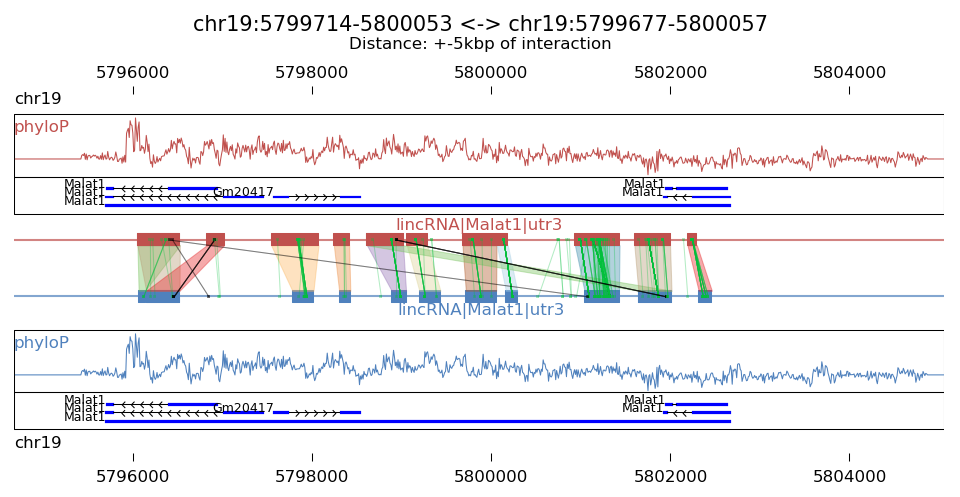
\includegraphics{local_interaction_malat1_ACCT.jpg}

\emph{Explanation:}


\chapter{Visualization of intra-RNA interactions by heatmap}
\label{Visualization:visualizationheatmap}\label{Visualization:visualization-of-intra-rna-interactions-by-heatmap}

\section{Prerequirement}
\label{Visualization:id1}
This program require python modules: xplib, matplotlib, numpy


\section{Run the program to generate heatmap for interactions within RNA molecule}
\label{Visualization:run-the-program-to-generate-heatmap-for-interactions-within-rna-molecule}
\index{Plot\_interaction\_heatmap.py}
This program could generate an heatmap to show interactions between different regions within an RNA molecule which are spatially proximate to each other. We use the script ``Plot\_interaction\_heatmap.py''

\begin{Verbatim}[commandchars=\\\{\}]
usage: Plot\_interaction\_heatmap.py [-h] [-n NAME] [-r R]
                                   [-s START [START ...]] [-g GENEBED]
                                   [-p PAIR\_DIST] [-S] [-t STEP] [-I]
                                   [-o OUTPUT]
                                   interaction linkedPair

plot interactions using a heatmap. information of linked pairs are stored in
file '*\_fragment\_paired\_align.txt'

positional arguments:
  interaction           Interaction file from output of
                        'Select\_strongInteraction\_pp.py'
  linkedPair            file for information of linked pairs, which is output
                        of 'Stitch-seq\_Aligner.py'

optional arguments:
  -h, --help            show this help message and exit
  -n NAME, --name NAME  give a gene name and plot the interaction heatmap new
                        the gene region, exclusive with '-r' option
  -r R                  Choose region to plot, give region with format 'chr
                        :start-end', exclusive with '-n' option
  -s START [START ...], --start START [START ...]
                        start column number of the second region in
                        interaction file and linkedPair file, default=(7,9)
  -g GENEBED, --genebed GENEBED
                        the genebed file from Ensembl, default:
                        Ensembl\_mm9.genebed
  -p PAIR\_DIST, --pair\_dist PAIR\_DIST
                        two interacted parts within this distance are
                        considered as self-ligated and they are marked or
                        eliminated (see option -s for slim mode), default:
                        1000bp
  -S, --Slim            set slim mode to eliminate self ligated interactions
  -t STEP, --step STEP  step or resolution or unit size of the heatmap,
                        default=10bp
  -I, --SI              Specify to add strong interaction in the
                        figure,default: False
  -o OUTPUT, --output OUTPUT
                        output plot file, can be format of emf, eps, pdf, png,
                        ps, raw, rgba, svg, svgz

Require: xplib, matplotlib, numpy
\end{Verbatim}

\begin{notice}{note}{Note:}
linkedPair file is the output *\_fragment\_paired\_align.txt from {\hyperref[Analysis_pipeline:step5]{\emph{Step5:Stitch-seq\_Aligner.py}}} of the pipeline; Interaction txt file is the output of {\hyperref[Analysis_pipeline:step6]{\emph{Step6:Select\_strongInteraction\_pp.py}}}. Users can use two different ways to give the region to be plotted. One is directly use the `-r' option to specify the region, another is to give a gene name and the script can find a larger region covering the gene region.
\end{notice}


\section{Example of result graph}
\label{Visualization:id2}
\emph{Example code:}

\begin{Verbatim}[commandchars=\\\{\}]
python Plot\_interaction\_heatmap.py
        ACCT\_GGCG\_interaction\_clusters.txt \PYGZbs{}
        ACCT\_GGCG\_fragment\_paired\_align\_rmRNA\_sort.txt.gz \PYGZbs{}
        -r chr9:120038418-120038722 \PYGZbs{}
        -t 5 \PYGZbs{}
        -s 7 9 \PYGZbs{}
        -g ../Data/Ensembl\_mm9.genebed.gz \PYGZbs{}
        -o Snora73\_intra\_interaction.pdf
\end{Verbatim}

\emph{Result figure:}

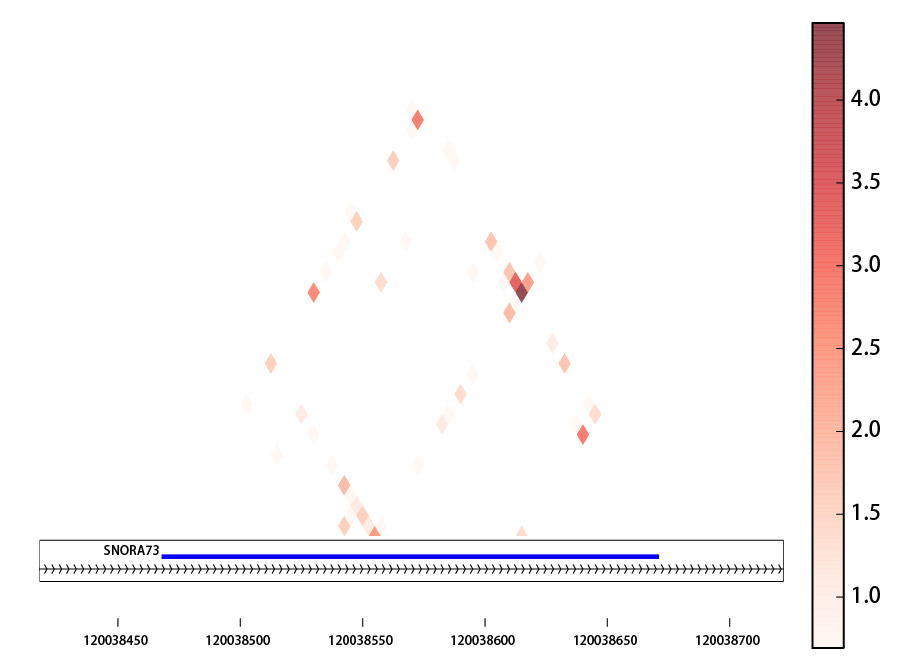
\includegraphics{Snora73_intra_interaction.jpg}

\emph{Explanation:}

The heatmap is basd on the log(count+1) of mapped linkage pairs across two windows with size {[}step{]}bp


\chapter{Visualization of global RNA-RNA interactome}
\label{Visualization:visualizationglobal}\label{Visualization:visualization-of-global-rna-rna-interactome}

\section{Prerequirement}
\label{Visualization:id3}
This program is powered by \href{http://cran.r-project.org/web/packages/RCircos/index.html}{RCircos}.

Required R packages (our program will check for the presence of these packages and install/load them automatically if not present):
\begin{itemize}
\item {} 
argparse, RCircos, biovizBase, rtracklayer

\end{itemize}

The program also require a python script ``bam2tab.py'' (already in /bin/ folder) to call coverage from \href{https://github.com/nimezhu/bam2x/blob/master/scripts/bed2tab.py}{BAM2X}


\section{Run the program to generate visualization}
\label{Visualization:id4}
\index{Plot\_Circos.R}
We will use the script ``Plot\_Circos.R'' for this purpose.

\begin{Verbatim}[commandchars=\\\{\}]
usage: Plot\_Circos.R [-h] [-g GENOME] [-b BIN] [-o OUTPUT]
                   interaction part1 part2

positional arguments:
  interaction           the interaction file,[required]
  part1                 aligned BAM file for part1,[required]
  part2                 aligned BAM file for part2,[required]

optional arguments:
  -h, --help            show this help message and exit
  -g GENOME, --genome GENOME
                        genome information, choice: mm9/mm10/hg19 et.al.,
                        [default: mm9]
  -b BIN, --bin BIN     window size for the bins for coverage calling, [default: 100000.0]
  -o OUTPUT, --output OUTPUT
                        output pdf file name, [default: Interactome\_view.pdf]
\end{Verbatim}

\begin{notice}{note}{Note:}
part1, part2 BAM files are the ones generated from {\hyperref[Analysis_pipeline:step5]{\emph{Step5:Stitch-seq\_Aligner.py}}} of the pipeline; Interaction txt file is the output of {\hyperref[Analysis_pipeline:step6]{\emph{Step6:Select\_strongInteraction\_pp.py}}}.
\end{notice}


\section{Example of result graph}
\label{Visualization:id5}
\emph{Example code:}

\begin{Verbatim}[commandchars=\\\{\}]
Rscript Plot\_Circos.R GGCG\_interaction\_clusters.txt
  sort\_Paired1\_fragment\_GGCG.bam sort\_Paired2\_fragment\_GGCG.bam
  -b 100000 -o Interactome\_GGCG.pdf
\end{Verbatim}

\emph{Result figure:}

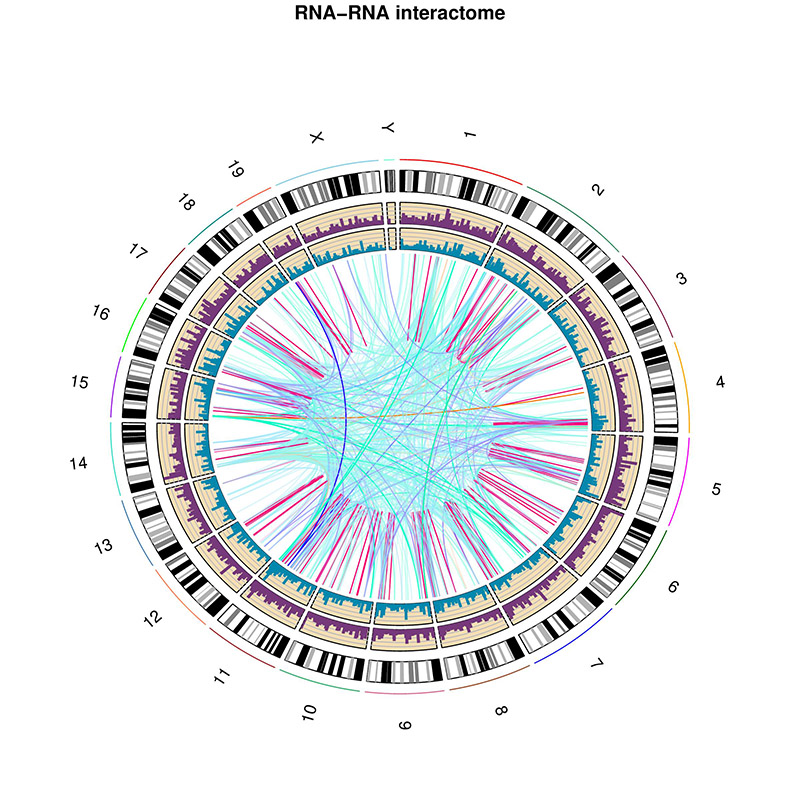
\includegraphics{GGCG-MEF_interactome.jpg}

\emph{Explanation:}


\chapter{Visualization of interaction types enrichment}
\label{Visualization:visualizationenrich}\label{Visualization:visualization-of-interaction-types-enrichment}

\section{Prerequirement}
\label{Visualization:id6}
Required R packages (our program will check for the presence of these packages and install/load them automatically if not present):
\begin{itemize}
\item {} 
``argparse'',''ggplot2'',''scales''

\end{itemize}


\section{Run the program to generate visualization for enrichment of different types of interactions}
\label{Visualization:run-the-program-to-generate-visualization-for-enrichment-of-different-types-of-interactions}
\index{Interaction\_type\_enrichment.R}
We will use the script ``Interaction\_type\_enrichment.R'' for this purpose.

\begin{Verbatim}[commandchars=\\\{\}]
usage: ../../bin/Interaction\_type\_enrichment.R [-h] [-n NUM [NUM ...]]
                                                [-o OUTPUT]
                                                interaction

 plot the statistical significance for enrichment of different interaction
 types

 positional arguments:
   interaction           the strong interaction file,[required]

 optional arguments:
   -h, --help            show this help message and exit
   -n NUM [NUM ...], --num NUM [NUM ...]
                         Column numbers for the type name in two part,[default:
                         [4, 11]]
   -o OUTPUT, --output OUTPUT
                         output pdf figure file, [default:
                         interaction\_type.pdf]
\end{Verbatim}

\begin{notice}{note}{Note:}
Interaction txt file is the output of {\hyperref[Analysis_pipeline:step6]{\emph{Step6:Select\_strongInteraction\_pp.py}}}.
\end{notice}


\section{Example of result graph}
\label{Visualization:id7}
\emph{Example code:}

\begin{Verbatim}[commandchars=\\\{\}]
Rscript Interaction\_type\_enrichment.R ACCT\_interaction\_clusters.txt
  -n 4 11 -o ACCT\_interaction\_type.pdf
\end{Verbatim}

\emph{Result figure:}

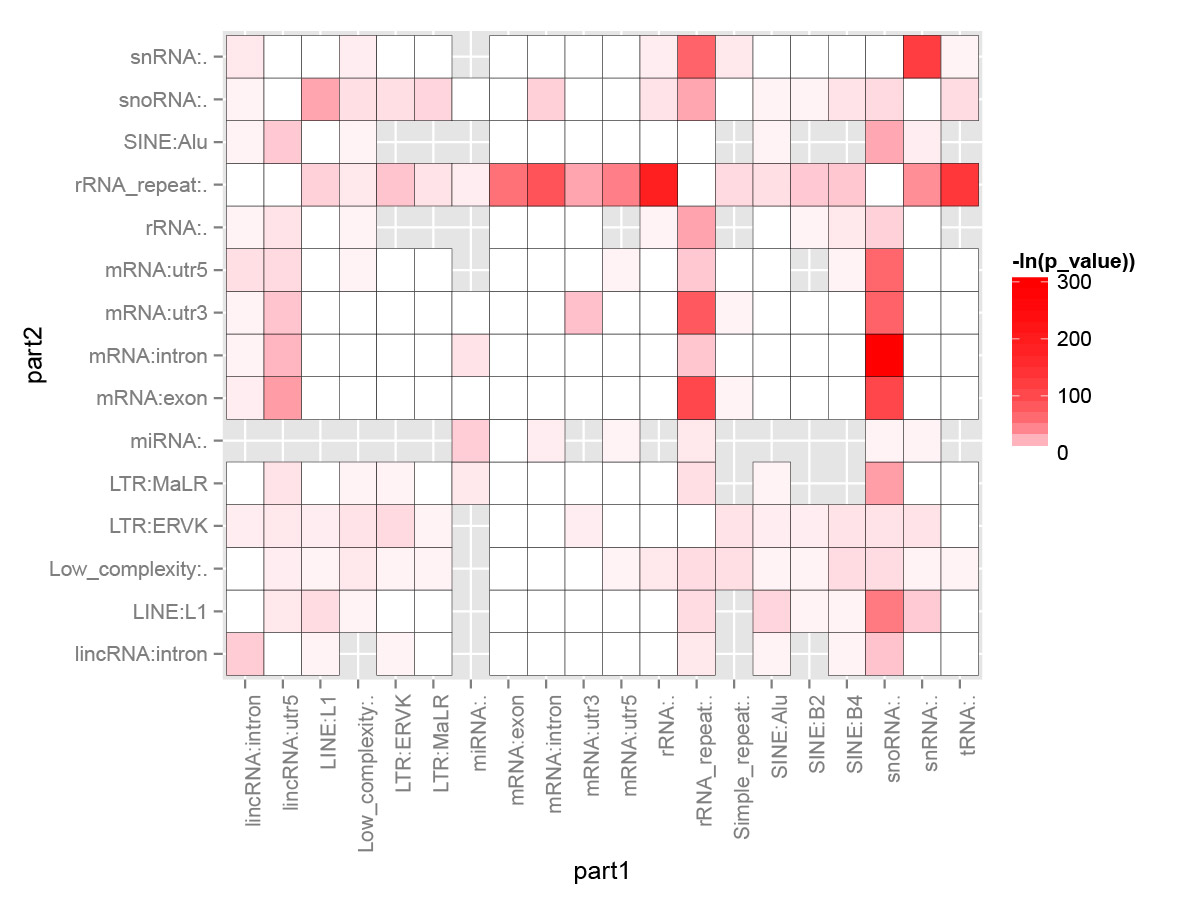
\includegraphics{ES1_interaction_type.jpg}

\emph{Explanation:}

For each interaction types (Type1\_in\_Part1\textless{}-\textgreater{}Type2\_in\_Part2), we calculated the number of Type1 in Part1 from all intereactions \code{n1} and number of Type2 in Part2 from all interactions \code{n2}. Then we calculate the number of interactions with this type: Type1\_in\_Part1\textless{}-\textgreater{}Type2\_in\_Part2 \code{n12}. The p-value for each interacction type is calculated based on the hypergeometric distribution with R command: \code{phyper(n12, n1, total\_n - n1, n2, lower.tail=F)}. Here \code{total\_n} is the total number of strong interactions. The color for each cell (each interaction type) are coded based on the value of ``-ln(p-value)''.


\chapter{Python APIs created for this project}
\label{Other_api:python-apis-created-for-this-project}\label{Other_api::doc}

\section{Annotation module}
\label{Other_api:annotation-module}\label{Other_api:module-Annotation}\index{Annotation (module)}
For the purpose of annotating RNA types for genomic regions.
\index{overlap() (in module Annotation)}

\begin{fulllineitems}
\phantomsection\label{Other_api:Annotation.overlap}\pysiglinewithargsret{\code{Annotation.}\bfcode{overlap}}{\emph{bed1}, \emph{bed2}}{}
This function compares overlap of two Bed object from same chromosome
\begin{quote}\begin{description}
\item[{Parameters}] \leavevmode\begin{itemize}
\item {} 
\textbf{bed1} -- A Bed object from \href{http://bam2xwiki.appspot.com/bed}{xplib.Annotation.Bed} (BAM2X)

\item {} 
\textbf{bed2} -- 
A Bed object from \href{http://bam2xwiki.appspot.com/bed}{xplib.Annotation.Bed} (BAM2X)


\end{itemize}

\item[{Returns}] \leavevmode
boolean -- True or False

\end{description}\end{quote}

Example:

\begin{Verbatim}[commandchars=\\\{\}]
\PYG{g+gp}{\PYGZgt{}\PYGZgt{}\PYGZgt{} }\PYG{k+kn}{from} \PYG{n+nn}{xplib.Annotation} \PYG{k+kn}{import} \PYG{n}{Bed}
\PYG{g+gp}{\PYGZgt{}\PYGZgt{}\PYGZgt{} }\PYG{k+kn}{from} \PYG{n+nn}{Annotation} \PYG{k+kn}{import} \PYG{n}{overlap}
\PYG{g+gp}{\PYGZgt{}\PYGZgt{}\PYGZgt{} }\PYG{n}{bed1}\PYG{o}{=}\PYG{n}{Bed}\PYG{p}{(}\PYG{p}{[}\PYG{l+s}{\PYGZdq{}}\PYG{l+s}{chr1}\PYG{l+s}{\PYGZdq{}}\PYG{p}{,}\PYG{l+m+mi}{10000}\PYG{p}{,}\PYG{l+m+mi}{12000}\PYG{p}{]}\PYG{p}{)}
\PYG{g+gp}{\PYGZgt{}\PYGZgt{}\PYGZgt{} }\PYG{n}{bed2}\PYG{o}{=}\PYG{n}{Bed}\PYG{p}{(}\PYG{p}{[}\PYG{l+s}{\PYGZdq{}}\PYG{l+s}{chr1}\PYG{l+s}{\PYGZdq{}}\PYG{p}{,}\PYG{l+m+mi}{9000}\PYG{p}{,}\PYG{l+m+mi}{13000}\PYG{p}{]}\PYG{p}{)}
\PYG{g+gp}{\PYGZgt{}\PYGZgt{}\PYGZgt{} }\PYG{k}{print} \PYG{n}{overlap}\PYG{p}{(}\PYG{n}{bed1}\PYG{p}{,}\PYG{n}{bed2}\PYG{p}{)}
\PYG{g+go}{True}
\end{Verbatim}

\end{fulllineitems}

\index{Subtype() (in module Annotation)}

\begin{fulllineitems}
\phantomsection\label{Other_api:Annotation.Subtype}\pysiglinewithargsret{\code{Annotation.}\bfcode{Subtype}}{\emph{bed1}, \emph{genebed}}{}
This function determines intron or exon or utr from a BED12 file.
\begin{quote}\begin{description}
\item[{Parameters}] \leavevmode\begin{itemize}
\item {} 
\textbf{bed1} -- 
A Bed object defined by \href{http://bam2xwiki.appspot.com/bed}{xplib.Annotation.Bed} (BAM2X)


\item {} 
\textbf{genebed} -- A Bed12 object representing a transcript defined by xplib Annotaton.Bed with information of exon/intron/utr from an BED12 file

\end{itemize}

\item[{Returns}] \leavevmode
str -- RNA subtype. ``intron''/''exon''/''utr3''/''utr5''/''.''

\end{description}\end{quote}

Example:

\begin{Verbatim}[commandchars=\\\{\}]
\PYG{g+gp}{\PYGZgt{}\PYGZgt{}\PYGZgt{} }\PYG{k+kn}{from} \PYG{n+nn}{xplib.Annotation} \PYG{k+kn}{import} \PYG{n}{Bed}
\PYG{g+gp}{\PYGZgt{}\PYGZgt{}\PYGZgt{} }\PYG{k+kn}{from} \PYG{n+nn}{xplib} \PYG{k+kn}{import} \PYG{n}{DBI}
\PYG{g+gp}{\PYGZgt{}\PYGZgt{}\PYGZgt{} }\PYG{k+kn}{from} \PYG{n+nn}{Annotation} \PYG{k+kn}{import} \PYG{n}{Subtype}
\PYG{g+gp}{\PYGZgt{}\PYGZgt{}\PYGZgt{} }\PYG{n}{bed1}\PYG{o}{=}\PYG{n}{Bed}\PYG{p}{(}\PYG{p}{[}\PYG{l+s}{\PYGZdq{}}\PYG{l+s}{chr13}\PYG{l+s}{\PYGZdq{}}\PYG{p}{,}\PYG{l+m+mi}{40975747}\PYG{p}{,}\PYG{l+m+mi}{40975770}\PYG{p}{]}\PYG{p}{)}
\PYG{g+gp}{\PYGZgt{}\PYGZgt{}\PYGZgt{} }\PYG{n}{a}\PYG{o}{=}\PYG{n}{DBI}\PYG{o}{.}\PYG{n}{init}\PYG{p}{(}\PYG{l+s}{\PYGZdq{}}\PYG{l+s}{../../Data/Ensembl\PYGZus{}mm9.genebed.gz}\PYG{l+s}{\PYGZdq{}}\PYG{p}{,}\PYG{l+s}{\PYGZdq{}}\PYG{l+s}{bed}\PYG{l+s}{\PYGZdq{}}\PYG{p}{)}
\PYG{g+gp}{\PYGZgt{}\PYGZgt{}\PYGZgt{} }\PYG{n}{genebed}\PYG{o}{=}\PYG{n}{a}\PYG{o}{.}\PYG{n}{query}\PYG{p}{(}\PYG{n}{bed1}\PYG{p}{)}\PYG{o}{.}\PYG{n}{next}\PYG{p}{(}\PYG{p}{)}
\PYG{g+gp}{\PYGZgt{}\PYGZgt{}\PYGZgt{} }\PYG{k}{print} \PYG{n}{Subtype}\PYG{p}{(}\PYG{n}{bed1}\PYG{p}{,}\PYG{n}{genebed}\PYG{p}{)}
\PYG{g+go}{\PYGZdq{}intron\PYGZdq{}}
\end{Verbatim}

\end{fulllineitems}

\index{annotation() (in module Annotation)}

\begin{fulllineitems}
\phantomsection\label{Other_api:Annotation.annotation}\pysiglinewithargsret{\code{Annotation.}\bfcode{annotation}}{\emph{bed}, \emph{ref\_allRNA}, \emph{ref\_detail}, \emph{ref\_repeat}}{}
This function is based on {\hyperref[Other_api:Annotation.overlap]{\code{overlap()}}} and {\hyperref[Other_api:Annotation.Subtype]{\code{Subtype()}}} functions to annotate RNA type/name/subtype for any genomic region.
\begin{quote}\begin{description}
\item[{Parameters}] \leavevmode\begin{itemize}
\item {} 
\textbf{bed} -- 
A Bed object defined by \href{http://bam2xwiki.appspot.com/bed}{xplib.Annotation.Bed} (in BAM2X).


\item {} 
\textbf{ref\_allRNA} -- the \href{http://bam2xwiki.appspot.com/DBI}{DBI.init} object (from BAM2X) for bed6 file of all kinds of RNA

\item {} 
\textbf{ref\_detail} -- 
the \href{http://bam2xwiki.appspot.com/DBI}{DBI.init} object for bed12 file of lincRNA and mRNA with intron, exon, UTR


\item {} 
\textbf{ref\_detail} -- 
the \href{http://bam2xwiki.appspot.com/DBI}{DBI.init} object for bed6 file of mouse repeat


\end{itemize}

\item[{Returns}] \leavevmode
list of str -- {[}type,name,subtype{]}

\end{description}\end{quote}

Example:

\begin{Verbatim}[commandchars=\\\{\}]
\PYG{g+gp}{\PYGZgt{}\PYGZgt{}\PYGZgt{} }\PYG{k+kn}{from} \PYG{n+nn}{xplib.Annotation} \PYG{k+kn}{import} \PYG{n}{Bed}
\PYG{g+gp}{\PYGZgt{}\PYGZgt{}\PYGZgt{} }\PYG{k+kn}{from} \PYG{n+nn}{xplib} \PYG{k+kn}{import} \PYG{n}{DBI}
\PYG{g+gp}{\PYGZgt{}\PYGZgt{}\PYGZgt{} }\PYG{k+kn}{from} \PYG{n+nn}{Annotation} \PYG{k+kn}{import} \PYG{n}{annotation}
\PYG{g+gp}{\PYGZgt{}\PYGZgt{}\PYGZgt{} }\PYG{n}{bed}\PYG{o}{=}\PYG{n}{Bed}\PYG{p}{(}\PYG{p}{[}\PYG{l+s}{\PYGZdq{}}\PYG{l+s}{chr13}\PYG{l+s}{\PYGZdq{}}\PYG{p}{,}\PYG{l+m+mi}{40975747}\PYG{p}{,}\PYG{l+m+mi}{40975770}\PYG{p}{]}\PYG{p}{)}
\PYG{g+gp}{\PYGZgt{}\PYGZgt{}\PYGZgt{} }\PYG{n}{ref\PYGZus{}allRNA}\PYG{o}{=}\PYG{n}{DBI}\PYG{o}{.}\PYG{n}{init}\PYG{p}{(}\PYG{l+s}{\PYGZdq{}}\PYG{l+s}{../../Data/all\PYGZus{}RNAs\PYGZhy{}rRNA\PYGZus{}repeat.txt.gz}\PYG{l+s}{\PYGZdq{}}\PYG{p}{,}\PYG{l+s}{\PYGZdq{}}\PYG{l+s}{bed}\PYG{l+s}{\PYGZdq{}}\PYG{p}{)}
\PYG{g+gp}{\PYGZgt{}\PYGZgt{}\PYGZgt{} }\PYG{n}{ref\PYGZus{}detail}\PYG{o}{=}\PYG{n}{DBI}\PYG{o}{.}\PYG{n}{init}\PYG{p}{(}\PYG{l+s}{\PYGZdq{}}\PYG{l+s}{../../Data/Ensembl\PYGZus{}mm9.genebed.gz}\PYG{l+s}{\PYGZdq{}}\PYG{p}{,}\PYG{l+s}{\PYGZdq{}}\PYG{l+s}{bed}\PYG{l+s}{\PYGZdq{}}\PYG{p}{)}
\PYG{g+gp}{\PYGZgt{}\PYGZgt{}\PYGZgt{} }\PYG{n}{ref\PYGZus{}repeat}\PYG{o}{=}\PYG{n}{DBI}\PYG{o}{.}\PYG{n}{init}\PYG{p}{(}\PYG{l+s}{\PYGZdq{}}\PYG{l+s}{../../Data/mouse.repeat.txt.gz}\PYG{l+s}{\PYGZdq{}}\PYG{p}{,}\PYG{l+s}{\PYGZdq{}}\PYG{l+s}{bed}\PYG{l+s}{\PYGZdq{}}\PYG{p}{)}
\PYG{g+gp}{\PYGZgt{}\PYGZgt{}\PYGZgt{} }\PYG{k}{print} \PYG{n}{annotation}\PYG{p}{(}\PYG{n}{bed}\PYG{p}{,}\PYG{n}{ref\PYGZus{}allRNA}\PYG{p}{,}\PYG{n}{ref\PYGZus{}detail}\PYG{p}{,}\PYG{n}{ref\PYGZus{}repeat}\PYG{p}{)}
\PYG{g+go}{[\PYGZdq{}protein\PYGZus{}coding\PYGZdq{},\PYGZdq{}gcnt2\PYGZdq{},\PYGZdq{}intron\PYGZdq{}]}
\end{Verbatim}

\end{fulllineitems}



\section{``annotated\_bed'' data class}
\label{Other_api:annotated-bed-data-class}\index{annotated\_bed (class in data\_structure)}

\begin{fulllineitems}
\phantomsection\label{Other_api:data_structure.annotated_bed}\pysiglinewithargsret{\strong{class }\code{data\_structure.}\bfcode{annotated\_bed}}{\emph{x=None}, \emph{**kwargs}}{}
To store, compare, cluster for the genomic regions with RNA annotation information. Utilized in the program {\hyperref[Analysis_pipeline:step6]{\emph{Select\_stronginteraction\_pp.py}}}
\index{Cluster() (data\_structure.annotated\_bed method)}

\begin{fulllineitems}
\phantomsection\label{Other_api:data_structure.annotated_bed.Cluster}\pysiglinewithargsret{\bfcode{Cluster}}{\emph{c}}{}
Store cluster information of self object
\begin{quote}\begin{description}
\item[{Parameters}] \leavevmode
\textbf{c} -- cluster index

\end{description}\end{quote}

Example:

\begin{Verbatim}[commandchars=\\\{\}]
\PYG{g+gp}{\PYGZgt{}\PYGZgt{}\PYGZgt{} }\PYG{n}{a}\PYG{o}{=}\PYG{n}{annotated\PYGZus{}bed}\PYG{p}{(}\PYG{n+nb}{chr}\PYG{o}{=}\PYG{l+s}{\PYGZdq{}}\PYG{l+s}{chr13}\PYG{l+s}{\PYGZdq{}}\PYG{p}{,}\PYG{n}{start}\PYG{o}{=}\PYG{l+m+mi}{40975747}\PYG{p}{,}\PYG{n}{end}\PYG{o}{=}\PYG{l+m+mi}{40975770}\PYG{p}{)}
\PYG{g+gp}{\PYGZgt{}\PYGZgt{}\PYGZgt{} }\PYG{n}{a}\PYG{o}{.}\PYG{n}{Cluster}\PYG{p}{(}\PYG{l+m+mi}{3}\PYG{p}{)}
\PYG{g+gp}{\PYGZgt{}\PYGZgt{}\PYGZgt{} }\PYG{k}{print} \PYG{n}{a}\PYG{o}{.}\PYG{n}{cluster}
\PYG{g+go}{3}
\end{Verbatim}

\begin{notice}{note}{Note:}
a.cluster will be the count information when a become a cluster object in {\hyperref[Analysis_pipeline:step6]{\emph{Select\_stronginteraction\_pp.py}}}
\end{notice}

\end{fulllineitems}

\index{Update() (data\_structure.annotated\_bed method)}

\begin{fulllineitems}
\phantomsection\label{Other_api:data_structure.annotated_bed.Update}\pysiglinewithargsret{\bfcode{Update}}{\emph{S}, \emph{E}}{}
Update the upper and lower bound of the cluster after adding segments using Union-Find.
\begin{quote}\begin{description}
\item[{Parameters}] \leavevmode\begin{itemize}
\item {} 
\textbf{S} -- start loc of the newly added genomic segment

\item {} 
\textbf{E} -- end loc of the newly added genomic segment

\end{itemize}

\end{description}\end{quote}

Example:

\begin{Verbatim}[commandchars=\\\{\}]
\PYG{g+gp}{\PYGZgt{}\PYGZgt{}\PYGZgt{} }\PYG{n}{a}\PYG{o}{=}\PYG{n}{annotated\PYGZus{}bed}\PYG{p}{(}\PYG{n+nb}{chr}\PYG{o}{=}\PYG{l+s}{\PYGZdq{}}\PYG{l+s}{chr13}\PYG{l+s}{\PYGZdq{}}\PYG{p}{,}\PYG{n}{start}\PYG{o}{=}\PYG{l+m+mi}{40975747}\PYG{p}{,}\PYG{n}{end}\PYG{o}{=}\PYG{l+m+mi}{40975770}\PYG{p}{)}
\PYG{g+gp}{\PYGZgt{}\PYGZgt{}\PYGZgt{} }\PYG{n}{a}\PYG{o}{.}\PYG{n}{Update}\PYG{p}{(}\PYG{l+m+mi}{40975700}\PYG{p}{,}\PYG{l+m+mi}{40975800}\PYG{p}{)}
\PYG{g+gp}{\PYGZgt{}\PYGZgt{}\PYGZgt{} }\PYG{k}{print} \PYG{n}{a}\PYG{o}{.}\PYG{n}{start}\PYG{p}{,} \PYG{n}{a}\PYG{o}{.}\PYG{n}{end}
\PYG{g+go}{40975700 40975800}
\end{Verbatim}

\end{fulllineitems}

\index{\_\_init\_\_() (data\_structure.annotated\_bed method)}

\begin{fulllineitems}
\phantomsection\label{Other_api:data_structure.annotated_bed.__init__}\pysiglinewithargsret{\bfcode{\_\_init\_\_}}{\emph{x=None}, \emph{**kwargs}}{}
Initiation example:

\begin{Verbatim}[commandchars=\\\{\}]
\PYG{g+gp}{\PYGZgt{}\PYGZgt{}\PYGZgt{} }\PYG{n+nb}{str}\PYG{o}{=}\PYG{l+s}{\PYGZdq{}}\PYG{l+s}{chr13  40975747        40975770        +       ATTAAG...TGA    protein\PYGZus{}coding  gcnt2   intron}\PYG{l+s}{\PYGZdq{}}
\PYG{g+gp}{\PYGZgt{}\PYGZgt{}\PYGZgt{} }\PYG{n}{a}\PYG{o}{=}\PYG{n}{annotated\PYGZus{}bed}\PYG{p}{(}\PYG{n+nb}{str}\PYG{p}{)}
\PYG{g+go}{or}
\PYG{g+gp}{\PYGZgt{}\PYGZgt{}\PYGZgt{} }\PYG{n}{a}\PYG{o}{=}\PYG{n}{annotated\PYGZus{}bed}\PYG{p}{(}\PYG{n+nb}{chr}\PYG{o}{=}\PYG{l+s}{\PYGZdq{}}\PYG{l+s}{chr13}\PYG{l+s}{\PYGZdq{}}\PYG{p}{,}\PYG{n}{start}\PYG{o}{=}\PYG{l+m+mi}{40975747}\PYG{p}{,}\PYG{n}{end}\PYG{o}{=}\PYG{l+m+mi}{40975770}\PYG{p}{,}\PYG{n}{strand}\PYG{o}{=}\PYG{l+s}{\PYGZsq{}}\PYG{l+s}{+}\PYG{l+s}{\PYGZsq{}}\PYG{p}{,}\PYG{n+nb}{type}\PYG{o}{=}\PYG{l+s}{\PYGZdq{}}\PYG{l+s}{protein\PYGZus{}coding}\PYG{l+s}{\PYGZdq{}}\PYG{p}{,}\PYG{p}{)}
\end{Verbatim}

\end{fulllineitems}

\index{\_\_lt\_\_() (data\_structure.annotated\_bed method)}

\begin{fulllineitems}
\phantomsection\label{Other_api:data_structure.annotated_bed.__lt__}\pysiglinewithargsret{\bfcode{\_\_lt\_\_}}{\emph{other}}{}
Compare two objects self and other when they are not \textbf{overlapped}
\begin{quote}\begin{description}
\item[{Parameters}] \leavevmode
\textbf{other} -- another \code{annotated\_bed} object

\item[{Returns}] \leavevmode
boolean -- ``None'' if overlapped.

\end{description}\end{quote}

Example:

\begin{Verbatim}[commandchars=\\\{\}]
\PYG{g+gp}{\PYGZgt{}\PYGZgt{}\PYGZgt{} }\PYG{n}{a}\PYG{o}{=}\PYG{n}{annotated\PYGZus{}bed}\PYG{p}{(}\PYG{n+nb}{chr}\PYG{o}{=}\PYG{l+s}{\PYGZdq{}}\PYG{l+s}{chr13}\PYG{l+s}{\PYGZdq{}}\PYG{p}{,}\PYG{n}{start}\PYG{o}{=}\PYG{l+m+mi}{40975747}\PYG{p}{,}\PYG{n}{end}\PYG{o}{=}\PYG{l+m+mi}{40975770}\PYG{p}{)}
\PYG{g+gp}{\PYGZgt{}\PYGZgt{}\PYGZgt{} }\PYG{n}{b}\PYG{o}{=}\PYG{n}{annotated\PYGZus{}bed}\PYG{p}{(}\PYG{n+nb}{chr}\PYG{o}{=}\PYG{l+s}{\PYGZdq{}}\PYG{l+s}{chr13}\PYG{l+s}{\PYGZdq{}}\PYG{p}{,}\PYG{n}{start}\PYG{o}{=}\PYG{l+m+mi}{10003212}\PYG{p}{,}\PYG{n}{end}\PYG{o}{=}\PYG{l+m+mi}{10005400}\PYG{p}{)}
\PYG{g+gp}{\PYGZgt{}\PYGZgt{}\PYGZgt{} }\PYG{k}{print} \PYG{n}{a}\PYG{o}{\PYGZgt{}}\PYG{n}{b}
\PYG{g+go}{False}
\end{Verbatim}

\end{fulllineitems}

\index{\_\_str\_\_() (data\_structure.annotated\_bed method)}

\begin{fulllineitems}
\phantomsection\label{Other_api:data_structure.annotated_bed.__str__}\pysiglinewithargsret{\bfcode{\_\_str\_\_}}{}{}
Use print function to output the cluster information (chr, start, end, type, name, subtype,cluster)

Example:

\begin{Verbatim}[commandchars=\\\{\}]
\PYG{g+gp}{\PYGZgt{}\PYGZgt{}\PYGZgt{} }\PYG{n+nb}{str}\PYG{o}{=}\PYG{l+s}{\PYGZdq{}}\PYG{l+s}{chr13  40975747        40975770        +       ATTAAG...TGA    protein\PYGZus{}coding  gcnt2   intron}\PYG{l+s}{\PYGZdq{}}
\PYG{g+gp}{\PYGZgt{}\PYGZgt{}\PYGZgt{} }\PYG{n}{a}\PYG{o}{=}\PYG{n}{annotated\PYGZus{}bed}\PYG{p}{(}\PYG{n+nb}{str}\PYG{p}{)}
\PYG{g+gp}{\PYGZgt{}\PYGZgt{}\PYGZgt{} }\PYG{n}{a}\PYG{o}{.}\PYG{n}{Cluster}\PYG{p}{(}\PYG{l+m+mi}{3}\PYG{p}{)}
\PYG{g+gp}{\PYGZgt{}\PYGZgt{}\PYGZgt{} }\PYG{n}{a}\PYG{o}{.}\PYG{n}{Update}\PYG{p}{(}\PYG{l+m+mi}{40975700}\PYG{p}{,}\PYG{l+m+mi}{40975800}\PYG{p}{)}
\PYG{g+gp}{\PYGZgt{}\PYGZgt{}\PYGZgt{} }\PYG{k}{print} \PYG{n}{a}
\PYG{g+go}{\PYGZdq{}chr13  40975700        40975800        protein\PYGZus{}coding  gcnt2   intron  3\PYGZdq{}}
\end{Verbatim}

\end{fulllineitems}

\index{overlap() (data\_structure.annotated\_bed method)}

\begin{fulllineitems}
\phantomsection\label{Other_api:data_structure.annotated_bed.overlap}\pysiglinewithargsret{\bfcode{overlap}}{\emph{other}}{}
Find overlap between regions
\begin{quote}\begin{description}
\item[{Parameters}] \leavevmode
\textbf{other} -- another \code{annotated\_bed} object

\item[{Returns}] \leavevmode
boolean

\end{description}\end{quote}

\end{fulllineitems}


\end{fulllineitems}



\section{``RNAstructure'' class}
\label{Other_api:rnastructure-class}\label{Other_api:rnafold}\index{RNAstructure (class in RNAstructure)}

\begin{fulllineitems}
\phantomsection\label{Other_api:RNAstructure.RNAstructure}\pysiglinewithargsret{\strong{class }\code{RNAstructure.}\bfcode{RNAstructure}}{\emph{exe\_path=None}}{}
Interface class for \href{http://rna.urmc.rochester.edu/RNAstructure.html}{RNAstructure} executable programs.
\index{DuplexFold() (RNAstructure.RNAstructure method)}

\begin{fulllineitems}
\phantomsection\label{Other_api:RNAstructure.RNAstructure.DuplexFold}\pysiglinewithargsret{\bfcode{DuplexFold}}{\emph{seq1=None}, \emph{seq2=None}, \emph{dna=False}}{}
Use ``DuplexFold'' program to calculate the minimum folding between two input sequences
\begin{quote}\begin{description}
\item[{Parameters}] \leavevmode\begin{itemize}
\item {} 
\textbf{seq1,seq2} -- two DNA/RNA sequences as string, or existing fasta file name

\item {} 
\textbf{dna} -- boolean input. Specify then DNA parameters are to be used

\end{itemize}

\item[{Returns}] \leavevmode
minimum binding energy, (unit: kCal/Mol)

\end{description}\end{quote}

Example:

\begin{Verbatim}[commandchars=\\\{\}]
\PYG{g+gp}{\PYGZgt{}\PYGZgt{}\PYGZgt{} }\PYG{k+kn}{from} \PYG{n+nn}{RNAstructure} \PYG{k+kn}{import} \PYG{n}{RNAstructure}
\PYG{g+gp}{\PYGZgt{}\PYGZgt{}\PYGZgt{} }\PYG{n}{RNA\PYGZus{}prog} \PYG{o}{=} \PYG{n}{RNAstructure}\PYG{p}{(}\PYG{n}{exe\PYGZus{}path}\PYG{o}{=}\PYG{l+s}{\PYGZdq{}}\PYG{l+s}{/home/yu68/Software/RNAstructure/exe/}\PYG{l+s}{\PYGZdq{}}\PYG{p}{)}
\PYG{g+gp}{\PYGZgt{}\PYGZgt{}\PYGZgt{} }\PYG{n}{seq1} \PYG{o}{=} \PYG{l+s}{\PYGZdq{}}\PYG{l+s}{TAGACTGATCAGTAAGTCGGTA}\PYG{l+s}{\PYGZdq{}}
\PYG{g+gp}{\PYGZgt{}\PYGZgt{}\PYGZgt{} }\PYG{n}{seq2} \PYG{o}{=} \PYG{l+s}{\PYGZdq{}}\PYG{l+s}{GACTAGCTTAGGTAGGATAGTCAGTA}\PYG{l+s}{\PYGZdq{}}
\PYG{g+gp}{\PYGZgt{}\PYGZgt{}\PYGZgt{} }\PYG{n}{energy}\PYG{o}{=}\PYG{n}{RNA\PYGZus{}prog}\PYG{o}{.}\PYG{n}{DuplexFold}\PYG{p}{(}\PYG{n}{seq1}\PYG{p}{,}\PYG{n}{seq2}\PYG{p}{)}
\PYG{g+gp}{\PYGZgt{}\PYGZgt{}\PYGZgt{} }\PYG{k}{print} \PYG{n}{energy}
\end{Verbatim}

\end{fulllineitems}

\index{Fold() (RNAstructure.RNAstructure method)}

\begin{fulllineitems}
\phantomsection\label{Other_api:RNAstructure.RNAstructure.Fold}\pysiglinewithargsret{\bfcode{Fold}}{\emph{seq=None}, \emph{ct\_name=None}, \emph{sso\_file=None}, \emph{Num=1}}{}
Use ``Fold'' program to predict the secondary structure and output dot format.
\begin{quote}\begin{description}
\item[{Parameters}] \leavevmode\begin{itemize}
\item {} 
\textbf{seq} -- one DNA/RNA sequence as string, or existing fasta file name

\item {} 
\textbf{ct\_name} -- specify to output a ct file with this name, otherwise store in temp, default: None

\item {} 
\textbf{sso\_file} -- give a single strand offset file, format see \href{http://rna.urmc.rochester.edu/Text/File\_Formats.html\#Offset}{http://rna.urmc.rochester.edu/Text/File\_Formats.html\#Offset}

\item {} 
\textbf{Num} -- choose Num th predicted structure

\end{itemize}

\item[{Returns}] \leavevmode
dot format of RNA secondary structure and RNA sequence.

\end{description}\end{quote}

Example:

\begin{Verbatim}[commandchars=\\\{\}]
\PYG{g+gp}{\PYGZgt{}\PYGZgt{}\PYGZgt{} }\PYG{k+kn}{from} \PYG{n+nn}{RNAstructure} \PYG{k+kn}{import} \PYG{n}{RNAstructure}
\PYG{g+gp}{\PYGZgt{}\PYGZgt{}\PYGZgt{} }\PYG{n}{RNA\PYGZus{}prog} \PYG{o}{=} \PYG{n}{RNAstructure}\PYG{p}{(}\PYG{n}{exe\PYGZus{}path}\PYG{o}{=}\PYG{l+s}{\PYGZdq{}}\PYG{l+s}{/home/yu68/Software/RNAstructure/exe/}\PYG{l+s}{\PYGZdq{}}\PYG{p}{)}
\PYG{g+gp}{\PYGZgt{}\PYGZgt{}\PYGZgt{} }\PYG{n}{seq} \PYG{o}{=} \PYG{l+s}{\PYGZdq{}}\PYG{l+s}{AUAUAAUUAAAAAAUGCAACUACAAGUUCCGUGUUUCUGACUGUUAGUUAUUGAGUUAUU}\PYG{l+s}{\PYGZdq{}}
\PYG{g+gp}{\PYGZgt{}\PYGZgt{}\PYGZgt{} }\PYG{n}{sequence}\PYG{p}{,}\PYG{n}{dot}\PYG{o}{=}\PYG{n}{RNA\PYGZus{}prog}\PYG{o}{.}\PYG{n}{Fold}\PYG{p}{(}\PYG{n}{seq}\PYG{p}{)}
\PYG{g+gp}{\PYGZgt{}\PYGZgt{}\PYGZgt{} }\PYG{k}{assert}\PYG{p}{(}\PYG{n}{seq}\PYG{o}{==}\PYG{n}{sequence}\PYG{p}{)}
\end{Verbatim}

\end{fulllineitems}

\index{\_\_init\_\_() (RNAstructure.RNAstructure method)}

\begin{fulllineitems}
\phantomsection\label{Other_api:RNAstructure.RNAstructure.__init__}\pysiglinewithargsret{\bfcode{\_\_init\_\_}}{\emph{exe\_path=None}}{}
Initiation of object
\begin{quote}\begin{description}
\item[{Parameters}] \leavevmode
\textbf{exe\_path} -- the folder path of the RNAstructure executables

\end{description}\end{quote}

Example:

\begin{Verbatim}[commandchars=\\\{\}]
\PYG{g+gp}{\PYGZgt{}\PYGZgt{}\PYGZgt{} }\PYG{k+kn}{from} \PYG{n+nn}{RNAstructure} \PYG{k+kn}{import} \PYG{n}{RNAstructure}
\PYG{g+gp}{\PYGZgt{}\PYGZgt{}\PYGZgt{} }\PYG{n}{RNA\PYGZus{}prog} \PYG{o}{=} \PYG{n}{RNAstructure}\PYG{p}{(}\PYG{n}{exe\PYGZus{}path}\PYG{o}{=}\PYG{l+s}{\PYGZdq{}}\PYG{l+s}{/home/yu68/Software/RNAstructure/exe/}\PYG{l+s}{\PYGZdq{}}\PYG{p}{)}
\end{Verbatim}

\end{fulllineitems}

\index{scorer() (RNAstructure.RNAstructure method)}

\begin{fulllineitems}
\phantomsection\label{Other_api:RNAstructure.RNAstructure.scorer}\pysiglinewithargsret{\bfcode{scorer}}{\emph{ct\_name1}, \emph{ct\_name2}}{}
Use `scorer' pogram to compare a predicted secondary structure to an accepted structure. It calculates two quality metrics, sensitivity and PPV
\begin{quote}\begin{description}
\item[{Parameters}] \leavevmode\begin{itemize}
\item {} 
\textbf{ct\_name1} -- The name of a CT file containing predicted structure data.

\item {} 
\textbf{ct\_name2} -- The name of a CT file containing accepted structure data, can only store one structure.

\end{itemize}

\item[{Returns}] \leavevmode
sensitivity, PPV, number of the best predicted structure.

\end{description}\end{quote}

Example:

\begin{Verbatim}[commandchars=\\\{\}]
\PYG{g+gp}{\PYGZgt{}\PYGZgt{}\PYGZgt{} }\PYG{n}{ct\PYGZus{}name1} \PYG{o}{=} \PYG{l+s}{\PYGZdq{}}\PYG{l+s}{temp\PYGZus{}prediction.ct}\PYG{l+s}{\PYGZdq{}}
\PYG{g+gp}{\PYGZgt{}\PYGZgt{}\PYGZgt{} }\PYG{n}{ct\PYGZus{}name2} \PYG{o}{=} \PYG{l+s}{\PYGZdq{}}\PYG{l+s}{temp\PYGZus{}accept.ct}\PYG{l+s}{\PYGZdq{}}
\PYG{g+gp}{\PYGZgt{}\PYGZgt{}\PYGZgt{} }\PYG{k+kn}{from} \PYG{n+nn}{RNAstructure} \PYG{k+kn}{import} \PYG{n}{RNAstructure}
\PYG{g+gp}{\PYGZgt{}\PYGZgt{}\PYGZgt{} }\PYG{n}{RNA\PYGZus{}prog} \PYG{o}{=} \PYG{n}{RNAstructure}\PYG{p}{(}\PYG{n}{exe\PYGZus{}path}\PYG{o}{=}\PYG{l+s}{\PYGZdq{}}\PYG{l+s}{/home/yu68/Software/RNAstructure/exe/}\PYG{l+s}{\PYGZdq{}}\PYG{p}{)}
\PYG{g+gp}{\PYGZgt{}\PYGZgt{}\PYGZgt{} }\PYG{n}{sensitivity}\PYG{p}{,} \PYG{n}{PPV}\PYG{p}{,} \PYG{n}{Number} \PYG{o}{=} \PYG{n}{RNA\PYGZus{}prog}\PYG{o}{.}\PYG{n}{scorer}\PYG{p}{(}\PYG{n}{ct\PYGZus{}name1}\PYG{p}{,}\PYG{n}{ct\PYGZus{}name2}\PYG{p}{)}
\end{Verbatim}

\end{fulllineitems}


\end{fulllineitems}



\chapter{Resources of strong interactions from two mouse cell types}
\label{Data_Resources:resource}\label{Data_Resources::doc}\label{Data_Resources:resources-of-strong-interactions-from-two-mouse-cell-types}

\section{Description of different samples}
\label{Data_Resources:description-of-different-samples}

\subsection{E14-1}
\label{Data_Resources:e14-1}\begin{quote}\begin{description}
\item[{Cell line}] \leavevmode
ESC E14

\item[{Barcode}] \leavevmode
ACCT

\item[{Experimental Details}] \leavevmode
Actively growing E14 cells were UV irradiated (254 nm) at 200mJ/cm
to crosslink proteins to interacting RNAs. After cell lysis, we trim down RNAs into
1000-2000 nt using RNase I and remove DNA by TURBO DNase. To recover RNAs bound to
RNA-binding proteins, we biotin-labeled them with EZ-Link Iodoacetyl-PEG2-Biotin from
Pierce. RNA-protein complexes were next immobilized on Streptavidin-coated beads. The
beads are then saturated with free biotin, preventing it from interfering with following
ligation with biotin-tagged linker. A biotin-tagged RNA linker was ligated to the 5’-end
of immobilized RNAs. Proximity ligation was then carried out under diluted conditions
while the RNA-protein complexes are still bound on bead. After RNA purification by
Proteinase K and phenol-chloroform extraction, we specifically removed the unligated
biotin by first anneal a complementary DNA oligo to the biotin-tagged linker by using
the annealing protocol: 70oC for 5 min, 25oC for 20 min, T7 Exo for 30 min. Exonuclease
T7 was added to remove terminal unligated biotin at the double-stranded RNAlinker-DNAoligo
hybrid. T7 Exonuclease acts in the 5' to 3' direction, catalyzing the removal of 5'
mononucleotides from duplex DNA and RNA/DNA hybrids in the 5’ to 3’ direction. The resulted
RNAs were fragmented again into \textasciitilde{}200 nt using RNase III RNA Fragmentation Module from NEB
(1ul of RNase III in 6 min at 37C). The RNAs were purified by column and ligated with
sequencing adapter, then reverse-transcribed and PCR for library construction. We applied
an rRNA removal step after constructing cDNA by using an rRNA removal protocol based on
the Duplex-Specific thermostable nuclease (DSN) enzyme using the protocol recommended by
\href{http://supportres.illumina.com/documents/myillumina/7836bd3e-3358-4834-b2f7-80f80acb4e3f/dsn\_normalization\_sampleprep\_application\_note\_15014673\_c.pdf}{Illumina}.
The constructed cDNAs were quality-checked by Bioanalyzer. The cDNAs were next
subjected paired-end sequencing on HiSeq-2500 platform.

\item[{Linker}] \leavevmode
\emph{mL5}: 5' - rCrUrA rG/iBiodT/rA rGrCrC rCrArU rGrCrA rArUrG rCrGrA rGrGrA - 3'

\end{description}\end{quote}


\subsection{E14-2}
\label{Data_Resources:e14-2}\begin{quote}\begin{description}
\item[{Cell line}] \leavevmode
ESC E14

\item[{Barcode}] \leavevmode
GGCG

\item[{Experimental Details}] \leavevmode
Same as E14\_WP\_1 but this time rRNA removal was performed right after
Proteinase K and phenol-chloroform treatment using the GeneRead rRNA Depletion Kit by
Qiagen. Furthermore, the annealing of RNA linker and complementary DNA oligo was changed
into: denature for 90 s at 90°C, and then anneal at -0.1°C/s to 25 °C and then incubate
for 25 min at 25 °C. Since after rRNA depletion the amount of RNA remained was less than
that obtained from E14 \#1, we reduced the duration of RNA fragmentation by RNase III from
6 min to 3 min. However, this reduction in RNase III treatment led to large fragments than
desirable.

\item[{Linker}] \leavevmode
\emph{mL5}: 5' - rCrUrA rG/iBiodT/rA rGrCrC rCrArU rGrCrA rArUrG rCrGrA rGrGrA - 3'

\end{description}\end{quote}


\subsection{E14-indirect}
\label{Data_Resources:e14-indirect}\begin{quote}\begin{description}
\item[{Cell line}] \leavevmode
ESC E14

\item[{Barcode}] \leavevmode
AATG

\item[{Experimental Details}] \leavevmode
To detect interactions between RNAs that are not bound to the same protein
but to interacting proteins, we used formaldehyde in conjunction with a second crosslinker, EGS.
The combination of formaldehyde and EGS crosslinks both RNA-protein and protein-protein
interactions thereby maximize the detection of RNA-RNA interactions that are facilitated by
interacting proteins. Actively grown E14 cells was crosslinked with 1.5 mM of freshly prepared
EthylGlycol bis(SuccinimidylSuccinate) (EGS)) for 45 minutes at room temperature and then 1\% of
formaldehyde for 10 minutes also at room temperature. Since crosslinking by formaldehyde makes
the cells very rigid and less amenable to be broken down lysis buffer. Therefore, we utilized
sonication to fragment the protein-bound RNA into \textasciitilde{}1000 nt size range. The remaining steps were
performed similarly to E14\_WP\_2.

Another main difference between this sample and other samples is that we didn't remove the nuclei,
thus effectively including RNA-RNA interactions inside the nucleus into the sample. In other
samples, only the cytoplasm was enriched.

\item[{Linker}] \leavevmode
\emph{mL5}: 5' - rCrUrA rG/iBiodT/rA rGrCrC rCrArU rGrCrA rArUrG rCrGrA rGrGrA - 3'

\end{description}\end{quote}


\subsection{MEF}
\label{Data_Resources:mef}\begin{quote}\begin{description}
\item[{Cell line}] \leavevmode
MEF

\item[{Barcode}] \leavevmode
GGCG

\item[{Experimental Details}] \leavevmode
We irradiated actively grown 1E8 MEF cells (254 nm). This time, the RNAs
were fragmented into 300nt size range. RNase III fragmentation was also modified accordingly
to adjust for smaller amount of RNAs: instead of adding 1ul of RNase III, we added only 0.5uL
of RNase III and then incubated at 37C for 5 min. The subsequent steps were performed using
the same procedure as E14\_WP\_2.

\item[{Linker}] \leavevmode
\emph{mL5}: 5' - rCrUrA rG/iBiodT/rA rGrCrC rCrArU rGrCrA rArUrG rCrGrA rGrGrA - 3'

\end{description}\end{quote}


\section{Resources of Strong Interactions}
\label{Data_Resources:resources-of-strong-interactions}

\subsection{From merged data of E14-1 and E14-2:}
\label{Data_Resources:from-merged-data-of-e14-1-and-e14-2}

\subsubsection{Strong interactions based on clustering of genomic locations}
\label{Data_Resources:strong-interactions-based-on-clustering-of-genomic-locations}\begin{quote}\begin{description}
\item[{Genome}] \leavevmode
mm9

\item[{Explanation}] \leavevmode\begin{itemize}
\item {} 
First seven column is for information of cluster in Part1 of interaction (5'side of linker); second seven column is for information of cluster in Part2 of interaction (3'side of linker)

\item {} 
\textbf{Type}: RNA types or repeat types; \textbf{Name}: RNA or repeat names; \textbf{Subtype}: intron/utr3/utr5/exon for mRNA, intron/utr for lincRNA or repeat family; \textbf{Count}: number of supported reads in that cluster

\item {} 
Second last column is the number of mapped pairs that support this interaction.

\item {} 
Last column is the ``ln(p\_value)'' for the significance of interaction. P\_value is based on a hypergeometric test

\end{itemize}

\end{description}\end{quote}

\href{http://systemsbio.ucsd.edu/RNA-Hi-C/Data/ACCT\_GGCG\_interaction\_clusters.xlsx}{Strong interactions (ES\_UV)} (Include two sheets, one for all interactions, and another one for the interactions that are not involving rRNA)

\href{http://systemsbio.ucsd.edu/RNA-Hi-C/Data/ACCT\_GGCG\_cluster\_total\_sort.xlsx}{List of clusters (ES\_UV)} (Removing rRNA/rRNA\_repeats)

\href{http://systemsbio.ucsd.edu/RNA-Hi-C/Data/ACCT\_GGCG\_interaction\_clusters\_noLeftRight.xlsx}{Strong interactions noLeftRight (ES\_UV)} (Clusters are generated by merging RNA1 and RNA2, The directions of RNA1 and RNA2 are ignored)


\subsubsection{Strong interactions based on annotation of RNAs}
\label{Data_Resources:strong-interactions-based-on-annotation-of-rnas}\begin{quote}\begin{description}
\item[{Genome}] \leavevmode
mm9

\item[{Explanation}] \leavevmode\begin{itemize}
\item {} 
First six column is for information of RNA in Part1 of interaction (5'side of linker); second six column is for information of RNA in Part2 of interaction (3'side of linker)

\item {} 
\textbf{Type}: RNA or repeat types; \textbf{Name}: RNA or repeat names; \textbf{Count}: number of supported reads in that RNA

\item {} 
Second last column is the number of mapped pairs that support this interaction.

\item {} 
Last column is the ``ln(p\_value)'' for the significance of interaction. P\_value is based on a hypergeometric test

\end{itemize}

\end{description}\end{quote}

\href{http://systemsbio.ucsd.edu/RNA-Hi-C/Data/ACCT\_GGCG\_interaction\_clusters\_RNA.xlsx}{Strong interactions RNA (ES\_UV)}

\href{http://systemsbio.ucsd.edu/RNA-Hi-C/Data/ACCT\_GGCG\_interaction\_clusters\_RNA\_noLeftRight.xlsx}{Strong interactions RNA noLeftRight (ES\_UV)} (The directions of RNA1 and RNA2 are ignored, and interactions involving introns are deleted)


\subsubsection{Strong interactions based on annotation of RNAs (FDR and using ES-indirect as control)}
\label{Data_Resources:strong-interactions-based-on-annotation-of-rnas-fdr-and-using-es-indirect-as-control}\label{Data_Resources:sifdr}\begin{quote}\begin{description}
\item[{Genome}] \leavevmode
mm9

\item[{Explanation}] \leavevmode\begin{itemize}
\item {} 
First six column is for information of RNA in Part1 of interaction (5'side of linker); second six column is for information of RNA in Part2 of interaction (3'side of linker)

\item {} 
\textbf{Type}: RNA or repeat types; \textbf{Name}: RNA or repeat names; \textbf{Count}: number of supported reads in that RNA

\item {} 
Column 15 is the number of mapped pairs that support this interaction.

\item {} 
Column 16 is the ``ln(p\_value)'' for the significance of interaction. P\_value is based on a hypergeometric test, column 17 is p-value

\item {} 
Column 18 is the FDR. FDR is calculated using the Benjamini–Hochberg procedure

\item {} 
Column 19 is the fold change between merged data of ES14-1 and ES14-2 and dual crosslink data. The fold change is the ratio (\# of interaction in merged data + 0.5)/(\# of interaction in dual crosslink data + 0.5)

\end{itemize}

\end{description}\end{quote}

\href{http://systemsbio.ucsd.edu/RNA-Hi-C/Data/ACCT\_GGCG\_interaction\_cluster\_noLeftRight\_RNA\_DualCrosslinkControl\_significant.xlsx}{Strong interactions RNA noLeftRight FDR and using ES-indirect as control (ES\_UV)} (The directions of RNA1 and RNA2 are ignored, and interactions involving introns are deleted, using FDR cutoff and using ES-indirect as control)


\subsection{From E14-indirect dual crosslinking:}
\label{Data_Resources:from-e14-indirect-dual-crosslinking}

\subsubsection{Strong interactions based on clustering of genomic locations}
\label{Data_Resources:id1}\begin{quote}\begin{description}
\item[{Genome}] \leavevmode
mm9

\item[{Explanation}] \leavevmode\begin{itemize}
\item {} 
First seven column is for information of cluster in Part1 of interaction (5'side of linker); second seven column is for information of cluster in Part2 of interaction (3'side of linker)

\item {} 
\textbf{Type}: RNA types or repeat types; \textbf{Name}: RNA or repeat names; \textbf{Subtype}: intron/utr3/utr5/exon for mRNA, intron/utr for lincRNA or repeat family; \textbf{Count}: number of supported reads in that cluster

\item {} 
Second last column is the number of mapped pairs that support this interaction.

\item {} 
Last column is the ``ln(p\_value)'' for the significance of interaction. P\_value is based on a hypergeometric test

\end{itemize}

\end{description}\end{quote}

\href{http://systemsbio.ucsd.edu/RNA-Hi-C/Data/AATG\_interaction\_clusters.xlsx}{Strong interactions (ES\_indirect)} (Include two sheets, one for all interactions, and another one for the interactions that are not involving rRNA)

\href{http://systemsbio.ucsd.edu/RNA-Hi-C/Data/AATG\_cluster\_total\_sort.xlsx}{List of clusters (ES\_indirect)} (Removing rRNA/rRNA\_repeats)

\href{http://systemsbio.ucsd.edu/RNA-Hi-C/Data/AATG\_interaction\_clusters\_noLeftRight.xlsx}{Strong interactions noLeftRight (ES\_indirect)} (Clusters are generated by merging RNA1 and RNA2, The directions of RNA1 and RNA2 are ignored)


\subsubsection{Strong interactions based on annotation of RNAs}
\label{Data_Resources:id2}\begin{quote}\begin{description}
\item[{Genome}] \leavevmode
mm9

\item[{Explanation}] \leavevmode\begin{itemize}
\item {} 
First six column is for information of RNA in Part1 of interaction (5'side of linker); second six column is for information of RNA in Part2 of interaction (3'side of linker)

\item {} 
\textbf{Type}: RNA or repeat types; \textbf{Name}: RNA or repeat names; \textbf{Count}: number of supported reads in that RNA

\item {} 
Second last column is the number of mapped pairs that support this interaction.

\item {} 
Last column is the ``ln(p\_value)'' for the significance of interaction. P\_value is based on a hypergeometric test

\end{itemize}

\end{description}\end{quote}

\href{http://systemsbio.ucsd.edu/RNA-Hi-C/Data/AATG\_interaction\_clusters\_RNA.xlsx}{Strong interactions RNA (ES\_indirect)}

\href{http://systemsbio.ucsd.edu/RNA-Hi-C/Data/AATG\_interaction\_clusters\_RNA\_noLeftRight.xlsx}{Strong interactions RNA noLeftRight (ES\_indirect)} (The directions of RNA1 and RNA2 are ignored, and interactions involving introns are deleted)


\subsection{From MEF sample:}
\label{Data_Resources:from-mef-sample}

\subsubsection{Strong interactions based on clustering of genomic locations}
\label{Data_Resources:id3}\begin{quote}\begin{description}
\item[{Genome}] \leavevmode
mm9

\item[{Explanation}] \leavevmode\begin{itemize}
\item {} 
First seven column is for information of cluster in Part1 of interaction (5'side of linker); second seven column is for information of cluster in Part2 of interaction (3'side of linker)

\item {} 
\textbf{Type}: RNA types or repeat types; \textbf{Name}: RNA or repeat names; \textbf{Subtype}: intron/utr3/utr5/exon for mRNA, intron/utr for lincRNA or repeat family; \textbf{Count}: number of supported reads in that cluster

\item {} 
Second last column is the number of mapped pairs that support this interaction.

\item {} 
Last column is the ``ln(p\_value)'' for the significance of interaction. P\_value is based on a hypergeometric test

\end{itemize}

\end{description}\end{quote}

\href{http://systemsbio.ucsd.edu/RNA-Hi-C/Data/GGCG\_MEF\_interaction\_clusters.xlsx}{Strong interactions (MEF)} (Include two sheets, one for all interactions, and another one for the interactions that are not involving rRNA)

\href{http://systemsbio.ucsd.edu/RNA-Hi-C/Data/GGCG\_MEF\_cluster\_total\_sort.xlsx}{List of clusters (MEF)} (Removing rRNA/rRNA\_repeats)

\href{http://systemsbio.ucsd.edu/RNA-Hi-C/Data/GGCG\_MEF\_interaction\_clusters\_noLeftRight.xlsx}{Strong interactions noLeftRight (MEF)} (Clusters are generated by merging RNA1 and RNA2, The directions of RNA1 and RNA2 are ignored)


\subsubsection{Strong interactions based on annotation of RNAs}
\label{Data_Resources:id4}\begin{quote}\begin{description}
\item[{Genome}] \leavevmode
mm9

\item[{Explanation}] \leavevmode\begin{itemize}
\item {} 
First six column is for information of RNA in Part1 of interaction (5'side of linker); second six column is for information of RNA in Part2 of interaction (3'side of linker)

\item {} 
\textbf{Type}: RNA or repeat types; \textbf{Name}: RNA or repeat names; \textbf{Count}: number of supported reads in that RNA

\item {} 
Second last column is the number of mapped pairs that support this interaction.

\item {} 
Last column is the ``ln(p\_value)'' for the significance of interaction. P\_value is based on a hypergeometric test

\end{itemize}

\end{description}\end{quote}

\href{http://systemsbio.ucsd.edu/RNA-Hi-C/Data/GGCG\_MEF\_interaction\_clusters\_RNA.xlsx}{Strong interactions RNA (MEF)}

\href{http://systemsbio.ucsd.edu/RNA-Hi-C/Data/GGCG\_MEF\_interaction\_clusters\_RNA\_noLeftRight.xlsx}{Strong interactions RNA noLeftRight (MEF)} (The directions of RNA1 and RNA2 are ignored, and interactions involving introns are deleted)


\subsection{Number of different types of interactions:}
\label{Data_Resources:number-of-different-types-of-interactions}
\href{http://systemsbio.ucsd.edu/RNA-Hi-C/Data/Count\_types\_interaction\_fragment.htm}{Strong interactions based on clusters of genomic locations} (There are three sheets, ``All\_interactions'', ``Inter-RNA\_interactions'', ``Intra-RNA interactions'')

\href{http://systemsbio.ucsd.edu/RNA-Hi-C/Data/Count\_types\_interaction\_fragment\_wholeRNA.htm}{Strong interactions based on annotations of RNAs}

\href{http://systemsbio.ucsd.edu/RNA-Hi-C/Data/Count\_types\_interaction\_fragment\_wholeRNA\_noLeftRight.htm}{Strong interactions based on annotations of RNAs noLeftRight no Intron}
\begin{itemize}
\item {} 
For each cell type, there are two columns,

\item {} 
The first column gives the number of strong interactions with this interaction type,

\item {} 
the second column gives the number of mapped pairs that support this interaction type.

\end{itemize}


\section{Target of miRNA in mir-290-295 clusters and mmu-mir-703}
\label{Data_Resources:target-of-mirna-in-mir-290-295-clusters-and-mmu-mir-703}\begin{itemize}
\item {} 
The information of miRNAs are in columns 1-5;

\item {} 
The information of target locations are in columns 6-11;

\item {} 
The the last column gives the count of supported mapped pairs.

\end{itemize}


\subsection{From merged data of E14-1 and E14-2:}
\label{Data_Resources:id5}
\href{http://systemsbio.ucsd.edu/RNA-Hi-C/Data/ACCT\_GGCG\_interaction\_clusters\_miRNA.xlsx}{Target of miRNA in mir-290-295 clusters and mmu-mir-703 (ES\_UV)}


\subsection{From E14-indirect dual crosslinking:}
\label{Data_Resources:id6}
\href{http://systemsbio.ucsd.edu/RNA-Hi-C/Data/AATG\_interaction\_clusters\_miRNA.xlsx}{Target of miRNA in mir-290-295 clusters and mmu-mir-703 (ES\_dual)}

\begin{notice}{note}{Note:}
RNA Hi-C tools benifits a lot from BAM2X, a convenient python interface for most common NGS datatypes. \href{http://www.bam2x.net/}{Try BAM2X now}!
\end{notice}


\chapter{Updates}
\label{index:updates}\begin{description}
\item[{2014-6-27:}] \leavevmode\begin{itemize}
\item {} 
new strong interaction list added based on whole RNA annotation using a FDR cutoff, and using ES-indirect (dual crosslinking) sample as control. See: {\hyperref[Data_Resources:sifdr]{\emph{resources}}}, update in ``{\hyperref[Analysis_pipeline:step6]{\emph{Select\_strongInteraction\_pp.py}}}'' as well.

\end{itemize}

\item[{2014-5-15:}] \leavevmode\begin{itemize}
\item {} 
Add result {\hyperref[Data_Resources:resource]{\emph{resources}}} for identified strong interactions in mouse E14 cells and MEF cells.

\item {} 
New function to generate heatmap for intra-RNA interactions: {\hyperref[Visualization:visualizationheatmap]{\emph{Plot\_interaction\_heatmap.py}}}.

\end{itemize}

\item[{2014-05-14:}] \leavevmode\begin{itemize}
\item {} 
Add new function to find overlap between two interaction sets based on their RNA annotations, see: {\hyperref[Analysis_pipeline:intersectiongene]{\emph{intersectInteraction\_genePair.R}}}.

\item {} 
Allow input of two genomic regions to visualize local interactions using \code{-r} option in ``{\hyperref[Visualization:plotinteraction]{\emph{Plot\_interaction.py}}}'' function

\end{itemize}

\item[{2014-05-11:}] \leavevmode\begin{itemize}
\item {} 
Add new function to show enrichment of different types of interactions: {\hyperref[Visualization:visualizationenrich]{\emph{Interaction\_type\_enrichment.R}}}.

\end{itemize}

\item[{Version 0.3.2 (2014-05-07):}] \leavevmode\begin{itemize}
\item {} 
change the name into RNA-Hi-C

\end{itemize}

\item[{2014-05-06:}] \leavevmode\begin{itemize}
\item {} 
In ``{\hyperref[Analysis_pipeline:step6]{\emph{Select\_strongInteraction\_pp.py}}}'' function, now annotations are updated after doing clustering and for strong interaction. The indexing of annotation files may take some time.

\item {} 
New ``{\hyperref[Analysis_pipeline:structure]{\emph{RNA\_structure\_prediction.py}}}'' function to refine RNA structure prediction based on empirical offset of free energies for single strand nucleotide.

\end{itemize}

\item[{New features in 0.3.1 (2014-05-02):}] \leavevmode\begin{itemize}
\item {} 
Add ``--release'' option in ``{\hyperref[Analysis_pipeline:step4]{\emph{split\_partner.py}}}'' function. Allow a Type3 read-pair considered to be a ``Paired'' chimeric fragment even linker does not show up.

\item {} 
Fix bugs in ``{\hyperref[Analysis_pipeline:step6]{\emph{Select\_strongInteraction\_pp.py}}}'' function when the number of mapped pairs is low and some chromosomes don't have any mapped read in part1 or part2.

\item {} 
Add bowtie 2 option and Unique-align option in ``{\hyperref[Analysis_pipeline:step5]{\emph{Stitch-seq\_Aligner.py}}}'' function.

\item {} 
Different colors for different types of interactions in the {\hyperref[Visualization:visualizationglobal]{\emph{visualization of interactome}}}.

\item {} 
New API for folding energies of two RNA molecules, see ``{\hyperref[Other_api:rnafold]{\emph{RNAstructure}}}''.

\item {} 
Allow permutation-based strategies to calculate the p-value for the overlap between two independent interaction sets in ``{\hyperref[Analysis_pipeline:intersection]{\emph{intersectInteraction.py}}}'' function

\end{itemize}

\item[{New features in 0.2.2:}] \leavevmode\begin{itemize}
\item {} 
``{\hyperref[Visualization:plotinteraction]{\emph{Plot\_interaction.py}}}'' function to plot local RNA-RNA interactions.

\item {} 
``{\hyperref[Analysis_pipeline:intersection]{\emph{intersectInteraction.py}}}'' function to call overlap between two independent interaction sets.

\end{itemize}

\end{description}


\chapter{Indices and tables}
\label{index:indices-and-tables}\begin{itemize}
\item {} 
\emph{genindex}

\item {} 
\emph{modindex}

\item {} 
\emph{search}

\end{itemize}


\renewcommand{\indexname}{Python Module Index}
\begin{theindex}
\def\bigletter#1{{\Large\sffamily#1}\nopagebreak\vspace{1mm}}
\bigletter{a}
\item {\texttt{Annotation}}, \pageref{Other_api:module-Annotation}
\end{theindex}

\renewcommand{\indexname}{Index}
\printindex
\end{document}
